%-----------------------------------------------------------------------
% Template File for Science China Information Sciences
% Downloaded from http://scis.scichina.com
% Please compile the tex file using LATEX or PDF-LATEX or CCT-LATEX
%-----------------------------------------------------------------------

\documentclass{SCIS2021}
%%%%%%%%%%%%%%%%%%%%%%%%%%%%%%%%%%%%%%%%%%%%%%%%%%%%%%%
%%% Author's definitions for this manuscript
%%%%%%%%%%%%%%%%%%%%%%%%%%%%%%%%%%%%%%%%%%%%%%%%%%%%%%%

\usepackage{epstopdf}
\usepackage{graphicx}
\usepackage{graphbox}
\usepackage{indentfirst}
\usepackage{verbatim}
\usepackage{bm}
\usepackage{amssymb}
\usepackage{amsmath}
\usepackage{CJK}
\usepackage{xcolor,float}
\usepackage[subfigure]{tocloft}
\usepackage{subfig}


%\usepackage[algo2e]{algorithm2e}
\usepackage{algorithm}  
\usepackage{algorithmic} 
%\usepackage[noend]{algpseudocode}
%\usepackage{algorithmicx,algorithm}
\usepackage{booktabs}
\usepackage{multirow}
\usepackage{colortbl}
\usepackage{color}
\usepackage{array}
%\usepackage{ctex}
\usepackage{enumitem}
\usepackage{enumerate}
\usepackage{mathrsfs}





%%%%%%%%%%%%%%%%%%%%%%%%%%%%%%%%%%%%%%%%%%%%%%%%%%%%%%%
%%%%%%%%%%%%%%%%%%%%%%%%%%%%%%%%%%%%%%%%%%%%%%%%%%%%%%%
\begin{document}
	\bibliographystyle{unsrt}
	%%%%%%%%%%%%%%%%%%%%%%%%%%%%%%%%%%%%%%%%%%%%%%%%%%%%%%%
	%%% Authors do not modify the information below
	\ArticleType{RESEARCH PAPER}
	%\SpecialTopic{}
	\Year{}
	\Month{}
	\Vol{}
	\No{}
	\DOI{}
	\ArtNo{}
	\ReceiveDate{}
	\ReviseDate{}
	\AcceptDate{}
	\OnlineDate{}
	%%%%%%%%%%%%%%%%%%%%%%%%%%%%%%%%%%%%%%%%%%%%%%%%%%%%%%%
	
	%%% title: 
	%%%   \title{title}{title for citation}
	\title{Wireless/Wired Integrated Transmission for Industrial Cyber-physical Systems: Risk-sensitive Co-design of 5G and TSN Protocols}{}
	
	%%% Corresponding author: 
	%%%   \author[number]{Xinping GUAN}{{xpguan@sjtu.edu.cn}}
	%%% General author: 
	%%%   \author[number]{Full name}{}
	\author[1]{Yajing ZHANG}{}
	\author[2]{Qimin XU}{}
	\author[3]{Xinping GUAN}{xpguan@sjtu.edu.cn}
	\author[4]{Cailian CHEN}{}
	\author[5]{Mingyan LI}{}
	
	%%% Author information for page head. 
	\AuthorMark{Zhang Y J, et al.}
	
	%%% Authors for citation. 
	\AuthorCitation{Zhang Y J, Xu Q M, Guan X P, et al.}
	
	%%% Authors' contribution.
	\contributions{Authors 1 and 2 have the same contribution to this work.}
	
	%%% Address.
	%%%   \address[number]{Affiliation, City {\rm Postcode}, Country}
	%\address[1]{Affiliation, City {\rm 000000}, Country}
	\address{Department of Automation, Shanghai Jiao Tong University,\\ Key Laboratory of System Control and Information Processing, Ministry of Education of China, \\Shanghai 200240, P. R. China}
	%\address[3]{Affiliation, City {\rm 000000}, Country}
	
	%%% Abstract.
	\abstract{In order to realize intelligent manufacturing with a dynamic quality of service (QoS) for communication in industrial cyber-physical systems (ICPS), the deterministic transmission is needed in industrial networks by flexible access and reliable forwarding. For this reason, combining the 5th generation (5G) wireless communication technology with wired time-sensitive networking (TSN) technology is a promising solution. However, wireless communication adopted in the industry has characteristics such as diverse QoS of industrial data and complex signaling process, which bring the severe long tail of delay's distribution. These characteristics lead to the indeterminacy of wireless transmission. To address this issue, we propose a heterogeneous time-sensitive network (HTSN) co-designed by 5G and TSN in this paper. To provide hierarchical deterministic delivery in HTSN, a predictive multi-priority wireless scheduling mechanism is designed based on semi-persistent scheduling (SPS), and an adaptive data injection mechanism for TSN based on per-stream filtering and policing (PSFP). Considering the long tail of delay, we develop a risk-sensitive reinforcement learning strategy for realizing deterministic delivery. Simulations on a hot rolling production scenario demonstrate that HTSN with the proposed mechanisms achieves great performance in terms of the heterogeneous transmission. }
	
	%%% Keywords.
	\keywords{industrial cyber-physical systems (ICPS), 5G-TSN codesign, wireless/wired integrated network, risk-sensitive reinforcement learning, deterministic communication}
	
	\maketitle
	
	
	%%%%%%%%%%%%%%%%%%%%%%%%%%%%%%%%%%%%%%%%%%%%%%%%%%%%%%%
	%%% The main text.
	%%%%%%%%%%%%%%%%%%%%%%%%%%%%%%%%%%%%%%%%%%%%%%%%%%%%%%%
	\section{Introduction}
	\label{sec:introduction}
	{\color{blue}With the promotion of the fourth industrial revolution ( also known as industry 4.0 ), the manufacturing industry is converted from traditional industrial automation to intelligent manufacturing, where the latter integrates huge amounts of devices that embedded and networked together in industrial cyber physical system (ICPS)\cite{zhou2021temperature}. To improve the performance of intelligent manufacturing, such as real-time monitoring and control, deterministic communication is imperative from the industry field to the data center in order to provide real-time control for the control system. In particular, the automatic control system has a strict time demand, where the timely delivery of data is critical for intelligent manufacturing since violating a deadline may severely damage the control quality. However, the diversity of CPS applications deployed in industry field makes it intractable to meet their QoS demands\cite{zhou2020siamese}.}
	
	
	%提一下5G的握手时延很长,需要SPS进行资源预留
	\par As a new generation of wireless communication, the technology of 5G is expected to expand industrial informatics and automation into much broader contexts\cite{li2018predictive}. {\color{black}Among several typical usage} scenarios of 5G, ultra-reliable and low latency communication (URLLC) has the characteristics of high reliability up to 99.9999\% and low delay down to millisecond\cite{li2019learning}, which is appropriate for intelligent manufacturing, smart grid, and other automatic control scenarios. These scenarios require extremely high reliability {\color{black}as well as ultra low latency}. Besides, massive machine type communication (mMTC) is another target scenario for 5G, which is designed for monitoring and data collection in {\color{black}ICPS}. Unfortunately, there are three main problems to apply 5G technology to the {\color{black}ICPS}. (1) Due to the complex signaling process of the dynamic access mechanism, the conventional cellular network fails to guarantee the strict timelines of industrial automation. (2) The {\color{black}ICPS} has many characteristics such as the complex environment, limited radio resources, and severe interference, which lead to the long tail effect of delay distribution. (3) Data's QoS requirements are diverse and {\color{black}dynamica burst data always carries safety information}, which make it intractable to deliver data on demand.
	
	\par Contrary to the 5G technology, TSN standards ensure the determinacy and reliability of its innovative mechanisms such as gate control list (GCL) and time-aware shaper (TAS), which are suitable for {\color{black}URLLC} scenarios. Moreover, TSN gateways can deliver data in a guaranteed time window with bounded latency, small jitter, and extremely low data loss\cite{farkas20195g}. However, TSN is designed for standard ethernet, which has the inherent shortcomings of wired transmission, such as the limited coverage, the higher cost of maintenance, the complexity of installation, etc.
	
	\par Therefore, it is inevitable to propose a more flexible and deterministic transmission architecture to meet the requirements of intelligent manufacturing. {\color{black}To address this problem, we propose a heterogeneous architecture integrating 5G and TSN, named HTSN.} The contributions of this paper are summarized as follows.
	
	
	\begin{itemize}[itemsep=15pt,topsep=0pt]
		\item[(1)]
		\setlength{\itemsep}{15pt }
		\textbf{HTSN: {\color{black}a heterogeneous 5G-TSN integrated architecture}:}\\
		To provide flexible and deterministic transmission, we propose a heterogeneous architecture HTSN, in which the data flexibly accesses to the {\color{black}TSN gateway via 5G network and forwarded deterministically within TSN network}. Under this architecture, {\color{black}the data is delivered in time after two stages' adjustment in 5G and TSN, respectively.} 
	\end{itemize}
	
	\begin{itemize}[itemsep= 15pt,topsep =-0 pt]
		\item[(2)]
		\textbf{Predictive multi-priority wireless scheduling mechanism:}\\
		Considering the limited resources of {\color{black}ICPS}, we design a preemption based predictive multi-priority wireless scheduling mechanism on the basis of semi-persistent scheduling (SPS). {\color{black}In particular, limited resources are reserved for sensors according to their trigger correlations. Thus, the handshaking delay is reduced and the resource utilization is improved.}
	\end{itemize}
	
	\begin{itemize}[itemsep= 15pt,topsep = -0 pt]
		\item[(3)]
		\textbf{Adaptive data injection mechanism {\color{black}from 5G to TSN}:}\\
		{\color{black}To deal with the interference of industrial wireless environment, we propose an adaptive data injection mechanism based on the per-stream filtering and policing (PSFP) mechanism of TSN to offset the jitter caused by 5G communication. The relationship between the priority of queues and the transmission delay through TSN is given to adjust the priority of data while it is injected into TSN network.} 
	\end{itemize}
	
	\begin{itemize}[itemsep= 15 pt,topsep = -0 pt]
		\item[(4)]
		\textbf{Risk-sensitive learning stategy for wireless scheduling and data injection:}\\
		In consideration of the tail of the transmission delay, a risk-sensitive utility function is proposed, which consists of the expectation, variance, and third-order central moment of the total delay. Leveraging reinforcement learning to adjust the number of reserved resource blocks (RB) and the TSN injection queue, the delay distribution is more centralized with a shorter tail. Thus, the diverse QoS requirements of data are satisfied and the centralized delay distribution brings a more deterministic transmission.
	\end{itemize}
	
	{\color{blue}The remainder of this paper is organized as follows. In Section \ref{related}, we introduce the related work of heterogeneous network and real-time scheduling, then we give the overview of our HTSN in Section \ref{sec:Overview of HTSN}. In Section \ref{model}, we introduce the system model and formulate the optimization objective. Then we present the risk-sensitive learning strategy and simulation results in Section \ref{learning} and Section \ref{result}, respectively. Finally, this paper is concluded in Section \ref{con}.}
	
	%未标蓝版本表格
	\begin{comment}
	\begin{table}[htbp]
	\footnotesize
	\captionsetup{labelformat=empty}
	\caption{\textbf{List of Abbreviations}}
	\label{tal:abbreviation}
	\label{tab0}
	\tabcolsep 8pt %space between two columns.
	\begin{tabular*}{\textwidth}{c|c|c|c}
	\toprule
	\textbf{Full Name} & \textbf{Abbreviation} & \textbf{Full Name} & \textbf{Abbreviation} \\\hline
	QoS & Quality of Service & MTC & Machine Type Communication \\
	ICPS & Industrial Cyber Physical System & D2D & Device-to-Device \\
	5G & the 5th Generation wireless communication & IWN & Industrial Wireless Network\\
	TSN & Time-Sensitive Networking & BS & Base Station \\
	HTSN & Heterogeneous Time-Sensitive Networking architecture & NS & Non-Scheduled data \\
	SPS & Semi-Persistent Scheduling & TC & Time-Critical data \\
	PSFP & Per-Stream Filtering and Policing & BE & Best Effort data \\
	URLLC & Ultra-Reliable Low Latency Communication & TTI & Transmission Time Interval \\
	mMTC & massive Machine Type Communication & IPV & Internal Priority Values \\
	GCL & Gate Control List & MAB & Multi-Armed Bandits \\
	TAS & Time-Aware Shaper & RSL & Risk-Sensitive Learning \\
	E2E & End-to-End & GMAB & Gradient Multi-Armed Bandits \\
	SDN & Software-Defined Networking & MI & Mutual Information \\
	SR & Scheduling Request & X2 & Chi-Square Test \\
	SG & Scheduling Grant & SSA & Sensor Selection Algorithm \\
	\bottomrule
	\end{tabular*}
	\end{table}
	\end{comment}
	
	
	\begin{table}[htbp]
		\arrayrulecolor{blue}
		\footnotesize
		\captionsetup{labelformat=empty}
		\caption{{\color{blue}\textbf{List of Abbreviations}}}
		\label{tal:abbreviation}
		\label{tab0}
		\tabcolsep 8pt %space between two columns.
		\begin{tabular*}{\textwidth}{c|c|c|c}
			\toprule
			{\color{blue}\textbf{Full Name}} & {\color{blue}\textbf{Abbreviation}} & {\color{blue}\textbf{Full Name}} & {\color{blue}\textbf{Abbreviation}} \\\hline
			{\color{blue}QoS} & {\color{blue}Quality of Service} & {\color{blue}MTC} & {\color{blue}Machine Type Communication} \\
			{\color{blue}ICPS} & {\color{blue}Industrial Cyber Physical System} & {\color{blue}D2D} & {\color{blue}Device-to-Device} \\
			{\color{blue}5G} & {\color{blue}the 5th Generation wireless communication} & {\color{blue}IWN} & {\color{blue}Industrial Wireless Network}\\
			{\color{blue}TSN} & {\color{blue}Time-Sensitive Networking} & {\color{blue}BS} & {\color{blue}Base Station} \\
			{\color{blue}HTSN} & {\color{blue}Heterogeneous Time-Sensitive Networking architecture} & {\color{blue}NS} & {\color{blue}Non-Scheduled data} \\
			{\color{blue}SPS} & {\color{blue}Semi-Persistent Scheduling} & {\color{blue}TC} & {\color{blue}Time-Critical data} \\
			{\color{blue}PSFP} & {\color{blue}Per-Stream Filtering and Policing} & {\color{blue}BE} & {\color{blue}Best Effort data} \\
			{\color{blue}URLLC} & {\color{blue}Ultra-Reliable Low Latency Communication} & {\color{blue}TTI} & {\color{blue}Transmission Time Interval} \\
			{\color{blue}mMTC} & {\color{blue}massive Machine Type Communication} & {\color{blue}IPV} & {\color{blue}Internal Priority Values} \\
			{\color{blue}GCL} & {\color{blue}Gate Control List} & {\color{blue}MAB} & {\color{blue}Multi-Armed Bandits} \\
			{\color{blue}TAS} & {\color{blue}Time-Aware Shaper} & {\color{blue}RSL} & {\color{blue}Risk-Sensitive Learning} \\
			{\color{blue}E2E} & {\color{blue}End-to-End} & {\color{blue}GMAB} & {\color{blue}Gradient Multi-Armed Bandits} \\
			{\color{blue}SDN} & {\color{blue}Software-Defined Networking} & {\color{blue}MI} & {\color{blue}Mutual Information} \\
			{\color{blue}SR} & {\color{blue}Scheduling Request} & {\color{blue}X2} & {\color{blue}Chi-Square Test} \\
			{\color{blue}SG} & {\color{blue}Scheduling Grant} & {\color{blue}SSA} & {\color{blue}Sensor Selection Algorithm} \\
			\bottomrule
		\end{tabular*}
	\end{table}
	
	
	\section{Related Works}
	\label{related}
	The smart factory has received increasing attention for its strict communication demand of lower latency and higher reliability. The accompanying problem is how to improve the transmission determinacy of end-to-end (E2E) delay, which brings two main issues to focus on: the deterministic transmission via a heterogeneous network, the low access delay of the wireless network. Therefore, the related works are concluded in two aspects as mentioned above.
	
	
	\subsection{Heterogeneous Network Architecture}
	
	\subsubsection{Wireless/Wired Hybrid Network}
	In recent years, the combination of wireless and wired networks has attracted significant attantions \cite{fu2018software,ke2017improving,cai2006qos,underberg2018towards}. The authors in\cite{fu2018software,ke2017improving} concentrate on using software-defined networking (SDN) to provide centralized control of the wireless/wired network. \cite{fu2018software} proposes a network architecture where wireless and wired transmissions are used in parallel to make up for the shortcomings of the other one. \cite{ke2017improving} proposes a multi-path transmission mechanism under the architecture from wired to wireless to promote the video's transmission performance. Except for SDN, \cite{cai2006qos} proposes a protocol to support multimedia data in hybrid wireless/wired networks, which efficiently utilizes the wireless link with coexisting TCP flows and can provide satisfactory QoS for delay-sensitive multimedia applications. As for the industry, \cite{underberg2018towards} points out that since current wireless networks are not suitable to fulfill the applications' requirements, hybrid wired-wireless networks have to be developed in order to support the implementation of industrial CPS. However, these studies only focus on the hybrid transmission based on the traditional TCP/IP network while the coming 5G and TSN are more suitable for industrial communication.
	
	
	\subsubsection{5G-TSN Integrated Network}
	The TSN industry white paper recently points out that the URLLC scenario of 5G is the key to realizing the industrial internet. How to deeply combine 5G and TSN is the research hotspot. For this issue, Ericsson proposes a 5G-TSN integration conception in\cite{farkas20195g}, where the SDN controller manages the whole network, and TSN protocols are applied in 5G user planes to guarantee strict E2E delay. Furthermore, Ericsson thinks that the integration of URLLC in the manufacturing process has great potential to accelerate the transformation of the manufacturing industry\cite{sachs2019boosting}. Nevertheless, these combination of 5G and TSN are only preliminary ideas which still have a long way to be implemented.
	
	\subsection{Real-time Scheduling of Wireless Communications}
	
	\subsubsection{Risk-sensitive Transmission}~{}
	
	As stated in the introduction, the risk is a notion in financial mathenatics\cite{follmer2004stochastic}, which we want to resort to measuring the risk of transmission delay. For wireless communication, the risk is equivalent to the loss of valuable information due to the instability and randomness of wireless transmission. For example, the quality of the stochastic channel may cause a variation of latency, which will incur emergency information lost when the variation is higher\cite{batewela2019risk}. What's more, some fine-grained characteristics of delay in queueing networks, such as the delay distribution and probability boundary(the tail of delay), are critical while most works only care about the average delay rather than the worst delay\cite{bennis2018ultrareliable}. In existing works, \cite{yang2018low,vu2018path} study URLLC and low-latency communication to evaluate the performance under the influence of data dispersion and network density. They all focus on maximizing the average delay of network throughput or minimizing the average latency without providing any guarantee of the higher moment such as variance, skewness, kurtosis, etc. \cite{vu2017ultra}\cite{assaad2011risk} take the mean and variance of delay account to capture the tail of delay and optimize the bandwidth and transmission power without considering frequency diversity. To maximize the throughput of eMBB data, \cite{alsenwi2019embb} takes burst URLLC data into account and assumes it is a Rayleigh distribution, while the burst data is actually dynamic sporadic.
	
	\subsubsection{Semi-persisitent Scheduling}~{}
	
	Due to the complex "scheduling request-scheduling grant(SR-SG)" signaling mechanism, the conventional dynamic access scheme of the cellular network cannot satisfy the strict delay requirements\cite{holfeld2016wireless}. To this end, a fast uplink access scheme based on SPS is proposed in LTE Release 13\cite{3gpp2010}. Thus the uplink resources are assigned in advance to reduce the "SR-SG" overhead, which is suitable for machine-type communications (MTC) in industrial automation\cite{schulz2017latency}. However, SPS was designed for VoIP originally, the transmission of which is fixed and known, while the QoS of MTC devices varies, and the scheduling request is time-varying and even dynamic sporadic\cite{seo2012performance}. For this, \cite{afrin2015design} proposes an adaptive SPS scheme to adjust the resources in the next transmission by buffer report. Moreover, to make further use of unused resources, other devices can be assigned partial resources in a semi-persistent way based on device-to-device(D2D), which can lead to extra latency\cite{soleymani2016hierarchical}.
	
	\subsubsection{Multi-priority Wireless Transmission}~{}
	
	
	In the industrial wireless networks(IWNs), the priority of data can be established according to the requirements of applications\cite{raza2018novel}. Thus the essential requirement of IWNs is to support the transmission of mixed-priority data that have different demands of latency and reliability\cite{farag2018priority,gaj2012computer}. For example, as mentioned in\cite{zand2012wireless}, there are four different types of information in the industry: the safety/emergency information, which requires the highest reliability and the lowest latency, the regulate/monitor control information, which possesses the lenient requirements, the open-loop control information which allows minutes level delay and the monitoring information which has no requirements. To deal with this problem, \cite{lin2019framework} proposes a TDMA-based multichannel superframe strategy to keep the superiority of each priority with full radio channel reuse while the strategy is implemented for cluster-based IWN without considering burst data. Similarly, a multi-priority scheme named p-persistent is proposed in\cite{hang2020delay} based on CSMA, which guarantees the transmission of high priority at the expense of longer delay of low priority data and still doesn't take burst data into account.
	
	\par In conclusion, although optimizing wireless transmission have been well studied, it's still a big challenge to apply it to industrial automation.
	
	
	\section{Overview of HTSN}
	\label{sec:Overview of HTSN}
	As is illustrated in Figure~\ref{fig:The architecture of HTSN}, the architecture of HTSN consists of two coupling stages: the 5G network and the TSN network. The 5G network is composed of a set of $\mathcal{S}=\left(s_{1}, s_{2}, \ldots, s_{|S|}\right)$ sensors, communication nodes and controllers, etc. Different sensors collect different types of data. The TSN consists of a set of TSN gateways which also work as 5G base stations (BS). The BSs are in charge of the assignment of the RBs $\mathcal{R}=\left(r_{1}, r_{2}, \ldots, r_{|R|}\right)$, {\color{blue} where one RB denotes a series of time-frequency domains radio resource blocks and is sufficient to transmit most of the data collected by sensors. RB's corresponding time period, denoted by $\mathit{Subslot}$, is the minimum non-divisible time unit in 5G. The frequency band of one RB represents a channel, which is flat fading and homogeneous. In more detail, time-frequency resources of one RB mean that we can use the channel for a period of time (referred to as a $Subslot$ mentioned before).} {\color{black}RBs are shared indiscriminately by both SPS data and dynamic data.} The industrial field data from different sensors (temperature sensors, vibration sensors, etc.) is transmitted through shared RBs to TSN gateways, then is sent to the remote data center via wired TSN.
	
	%set a figure
	\begin{figure}[htb] 
		\centering 
		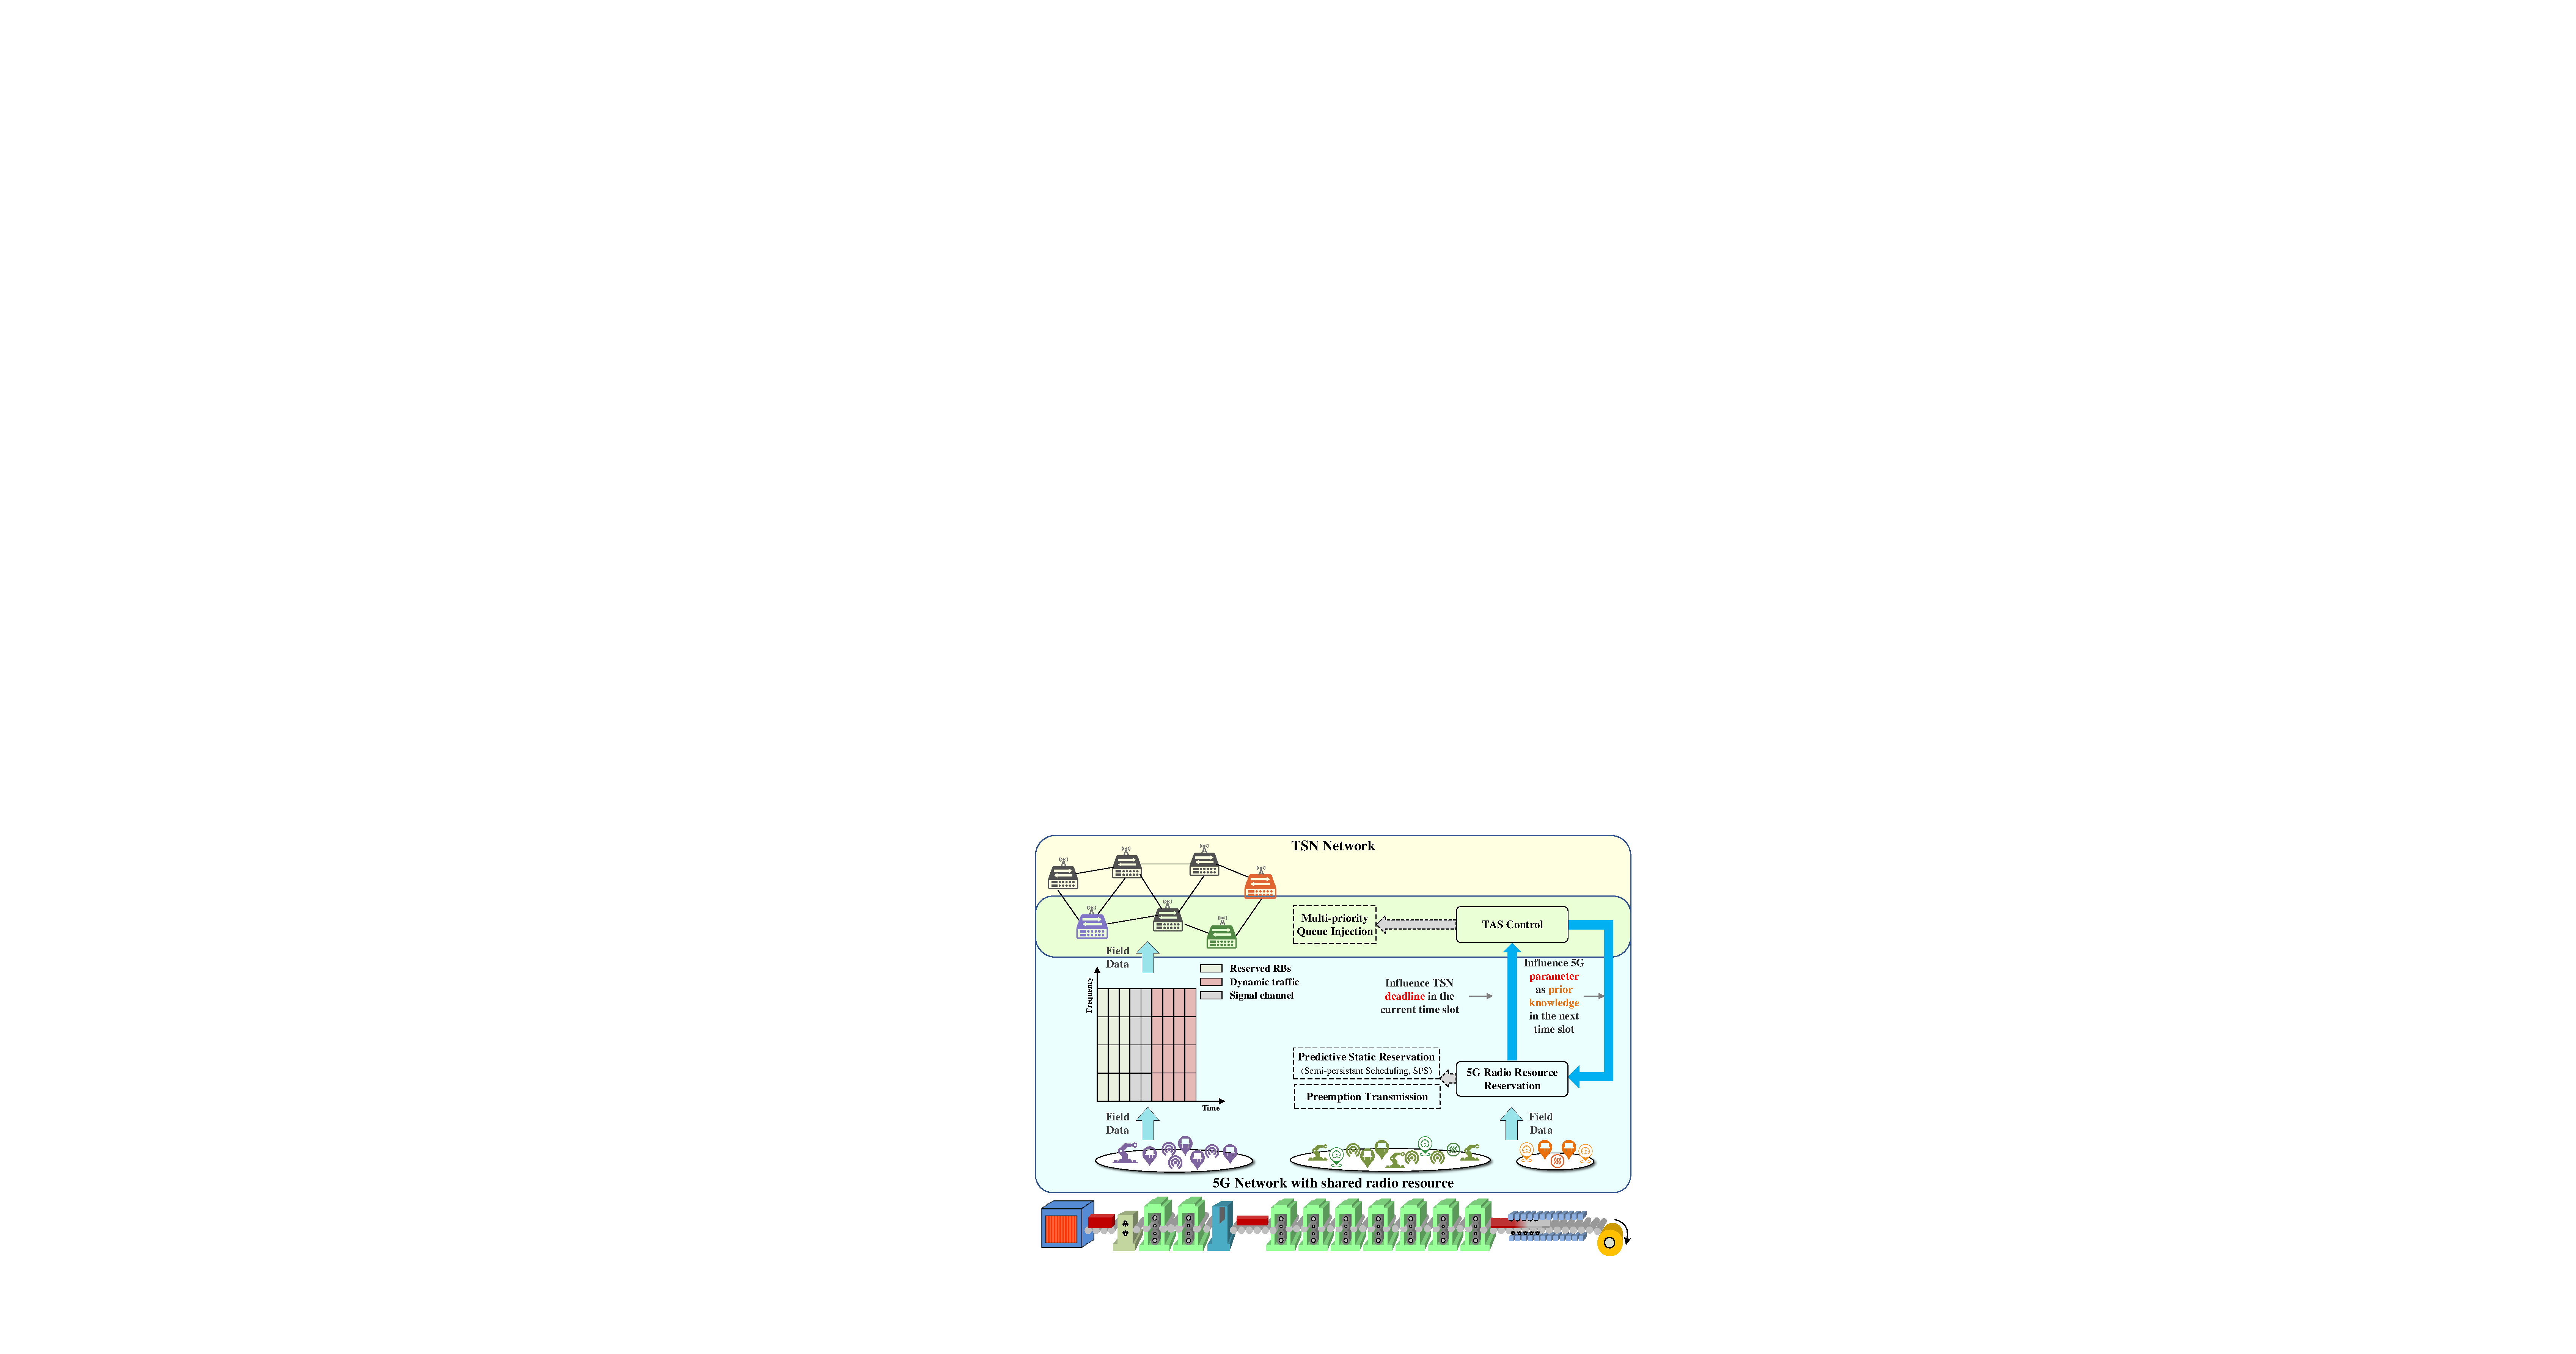
\includegraphics[height=9.5cm, width=13.8cm]{framework} 
		\caption{The architecture of HTSN} 
		\label{fig:The architecture of HTSN}
	\end{figure}
	
	\par Due to the diverse QoS requirements of field data, it is divided into three groups: (1) non-scheduled (NS) data, which is sporadically triggered by emergency data, and has the highest priority. (2) time-critical (TC) data, which is the primary type of data, and the amount of it is much larger than NS data. (3) best-effort (BE) data, which has the lowest priority and follows the best-effort forwarding rules. In industry, such as a hot rolling production process, data is transmitted periodically, and so we only consider the transmission in one time period of the 5G network, denoted by transmission time interval (TTI). The whole cycle of industrial automation can be regarded as the accumulation of TTIs. {\color{blue}In each TTI, we first select the node that are most likely to trigger, and then we transmit the TC data collected by these nodes on predictive reserved RBs based on SPS technique to omit handshaking delay. The residual TC data and BE data are served on dynamic RBs by the conventional dynamic access procedure orderly, which consists of handshaking in signaling procedure of transmission process. The difference between predictive reserved RBs and dynamic RBs is that the reserved RBs are assigned to sensors in advance without explicit SR-SG signalling procedure.} Considering the highest priority and the sporadically triggered feature of NS data, we set a fixed reserved RB at each subslot for possible NS data. To improve the utilization of RBs, the fixed reserved RBs can be used by TC data and BE data with no NS data arriving. And NS data can preempt any data as soon as it arrives. Note that the priority of NS data is the same as TC data after it is embedded in the 5G network. 
	
	\par {\color{black}Based on the PSFP mechanism in the IEEE 802.1Qci protocol, TSN gateways assign different Gate IDs to data according to their transmission delay in 5G and internal priority values (IPV), which is related to its QoS demands. Data arrived at the gateway are injected into the gateway's sending queue that matches its Gate ID assigned before. 
	%没有体现出根据数据QoS进行传输,没有解释清楚什么是时间敏感传输
	Thus, data from the 5G network is scheduled differentially in the TSN to meet their diverse QoS requirements and achieve time-sensitive transmission under HTSN.}
	
	\par {\color{blue}Specifically, the delay of the TC data (including arrived NS data) across 5G network and TSN network in TTI $t$, denoted by $T_\text{5G}(t)$ and  $T_\text{TSN}(t)$ respectively, are coupled. Note that the E2E delay of TC data from the industrial field to the  remote data center can be calculated as $T_\text{E2E}(t) = T_\text{5G}(t) + T_\text{TSN}(t)$.} In each TTI, the total amount of RBs is fixed, so that the larger amount of predictivel reserved RBs $\left|\mathcal{R}_\mathrm{r}(t)\right|$ in TTI $t$, the smaller the number of RBs for dynamic access. Note that $\left|\mathcal{R}_\mathrm{r}(t)\right|$ is much smaller than the number of sensors in field (i.e.,$\left|\mathcal{R}_\mathrm{r}(t)\right|\ll\left|\mathcal{S}\right|$). {\color{blue}If $T_\text{5G}(t)$ of TC data is larger than excepted, it should be injected into a high priority queue $Q(t)$ of TSN gateways to offset the time deviation caused by 5G stage. Otherwise, data that has low 5G delay can be injected into low priority TSN queue to reserve resources for other data. Here, we aim to minimize the E2E delay of TC data, so it is necessary to consider both the $T_\text{5G}(t)$ and the $T_\text{TSN}(t)$.}
	
	%改到这里
	
	\par \example{We take the rolling production process as an illustration. As shown in Figure~\ref{fig:The architecture of HTSN}, the 5G BS is installed in the TSN gateway as a local control center with learning ability. At the beginning of each TTI, the BS decides the number of reserved RBs according to the history data. Then sensors correlated with sensors activated before are assigned to predictive reserved RBs and execute signaling procedure in prior. {\color{black}After that, the residual sensors dynamic access BSs with handshaking delays, thus 5G delay $T_\text{5G}(t)$ can be calculated according to the transmission state in 5G. Based on $T_\text{5G}(t)$ and the QoS requirement of data, the BS decides the Gate ID of the TSN gateway queue that data will inject into.}} 
	
	
	
	%The examples at the bottom of the .tex file can help you when preparing your manuscript. We are appreciate your effort to follow our style~\cite{1,2}.
	
	\begin{comment}
	\begin{algorithm}
	%\floatname{algorithm}{Algorithm}
	\renewcommand{\algorithmicrequire}{\textbf{Input:}}
	\renewcommand{\algorithmicensure}{\textbf{Output:}}
	\footnotesize
	\caption{Transmission Interaction of 5G and TSN}
	\label{alg1}
	{\fontsize{10}{13}\selectfont
	\begin{algorithmic}[1]
	\REQUIRE Delay demand of TC data $T_\text{ddl}(t)$;
	\ENSURE  The number of reserved RBs in the next TTI  $\left|\mathcal{R}_{\mathrm{r}}(t+1)\right|$\\ \ \ \qquad The index of TSN Gateway's queue in the next TTI $Q(t+1)$
	\STATE $\left|\mathcal{R}_{\mathrm{r}}(1)\right| = 0, T_\text{E2E}(0) = 0$;
	\WHILE{$i \leq t $}
	\STATE $T_\text{5G}(i) = \bm{\mathcal{F}_{5G}}(\left|\mathcal{R}_{\mathrm{r}}(i)\right|, T_\text{E2E}(i-1))$\\
	%\STATE Calculate the time deviation between $T_\text{5G}(i)$ and $T_\text{ddl}(i)$\\
	\STATE $Q(i) = \bm{\mathcal{F}_{Q}}((T_\text{ddl}(i)-T_\text{5G}(i)) $\\
	\STATE $T_\text{TSN}(i) = \bm{\mathcal{F}_{TSN}}(T_\text{5G}(i), Q(i))$\\
	\STATE $T_\text{E2E}(i) = T_\text{E2E}(i-1) + T_\text{5G}(i) + T_\text{TSN}(i)$\
	\STATE Update $\left|\mathcal{R}_{\mathrm{r}}(i+1)\right|$\;
	\ENDWHILE
	\end{algorithmic}
	}
	\end{algorithm}
	\end{comment}
	
	
	
	%\noindent where $\bm{\mathcal{F}_{5G}}()$ is the function to calculate 5G network delay, $\bm{\mathcal{F}_{Q}}()$ is the function to determine TSN queue's priority, and $\bm{\mathcal{F}_{TSN}}()$ is the function to give TSN delay.
	
	\begin{comment}
	%set an algorithm
	\begin{algorithm}[t]
	\SetAlgoLined
	\KwIn{Delay demand of TC data $T_\text{ddl}(t)$}
	\KwOut{The delay of TSN $T_\text{TSN}(t)$,\\ \qquad\qquad\, The number of reserved RBs in the next TTI  $\left|\mathcal{R}_{\mathrm{r}, t+1}\right|$,\\ \qquad\qquad\, The priority of TSN Gateway's queue in the next TTI $Q_{t+1}$ \\} 
	\SetKwInput{Initialization}{Initialization}
	\Initialization{$\left|\mathcal{R}_{\mathrm{r}, 0}\right| = 0, Q_{0} = 0, T_\text{E2E}(0) = 0$}
	\SetKwInput{KwIn}{Input}
	\For{i = \rm1,2,...,$t$}{
	$T_\text{5G}(i) = \bm{\mathcal{F}}(\left|\mathcal{R}_{\mathrm{r}, i}\right|, T_\text{E2E}(i))$\\
	Calculate the time deviation between $T_\text{5G}(i)$ and $T_\text{ddl}(i)$\\
	$T_\text{TSN}(i) = \bm{\mathcal{F}}_{Q_{i}}(T_\text{ddl}(i)-T_\text{5G}(i))$\\
	$T_\text{E2E}(i) += T_\text{5G}(i) + T_\text{TSN}(i)$\
	
	Update $\left|\mathcal{R}_{\mathrm{r}, i}\right|, Q_{i} $\;
	}	
	\caption{Transmission Interaction of 5G and TSN}
	\end{algorithm}
	\end{comment}
	
	\section{System Model}
	\label{model}
	
	\subsection{Multi-priority Transmission Model Based on SPS}       
	\label{sssec:preemption} 
	{\color{black}As discussed in the previous section, there are three issues of 5G network: (1) predictive assign sensors that are the most correlated, (2) embed sensors obeying their diverse QoS requirements, (3) preemption of NS data. To this end, a preemption based predictive multi-priority scheduling mechanism is proposed in this section. The predictive sensor selection policy will be expounded in Section~\ref{sec:selection} later.}
	
	%\subsubsection{Multi-priority Scheduling Mechanism with Preemption Considered}~{}
	\par As mentioned before, in intelligent manufacturing, a massive amount of data with diverse QoS requirements is generating all the time, which should be served on their time demand. However, the complex uplink "SR-SG" signaling process brings extra delay for handshaking. As a solution, reserving RBs to correlated sensors in advance without a signaling procedure is a suitable way to reduce transmission time. {\color{black} Even so, the urgent and critical data may still have an additional queueing delay due to the shortage of the time-frequency radio resources in the factory. To this end, a preemption mechanism is proposed in this paper, which permits NS data to preempt TC data and BE data in order to realize no-wait transmission as soon as it arrives.}
	
	
	
	\par {\color{black}According to the QoS demands of data, we split radio resources into four parts in time order: predictive reserved RBs $\mathcal{R}_{\text{r}} \left(\mathcal{R}_{\text {r}} \subset \mathcal{R}\right)$, referred to as reservation area $ \to$ RBs for signaling transmission $\to$ RBs to transmit TC data $\to$ RBs to transmit BE data, as shown in Figure~\ref{fig:RBs}. Taking NS data that carries safety information into account, we set one fixed reserved RB delicated to NS data at each subslot. }%The fixed reserved RBs overlap four parts, and so the longest delay of TC data is less than or equal to $2*Subslot$. 
	There comes a proplem: what if the NS data arrives while the fixed reserved RB has been allocated to the other data already? {\color{black}That should be discussed according to whether the assigned sensor is triggered in Table~\ref{tal:preemption}, where $r_{\text{brt},i}(t)$ denotes fixed reserved RB at $i$-th subslot of TTI $t$, $s_{i}(t)$ denotes the sensor assigned to $r_{\text{brt},i}(t)$, $\varphi(t)=\sum_{i=1}^{\left|\mathcal{R}_{\mathbf{r}}(t)\right| / \left|C\right|} \varphi_{i}$ denotes the number of fixed reserved RBs in reservation area, to which the sensors assigned are triggered;  $\zeta(t)=\sum_{i=1}^{\left|\mathcal{R}_{\mathbf{r}}(t)\right| / \left|C\right|} \zeta_{i}$ denotes the number of arrived NS data in reservation area and $\gamma(t)=\sum_{i=1}^{\left|\mathcal{R}_{\mathbf{r}}(t)\right| / \left|C\right|} \gamma_{i}$ denotes the number of fixed reserved RBs that is preempted by NS data while sensors assigned to them are triggered as well. Note that $C = \{c_{1},c_{2},c_{3}...\}$ is the set of channels and the number of channels is $|C|$.}
	
	\begin{figure}[t] 
		\flushright
		%\centering 
		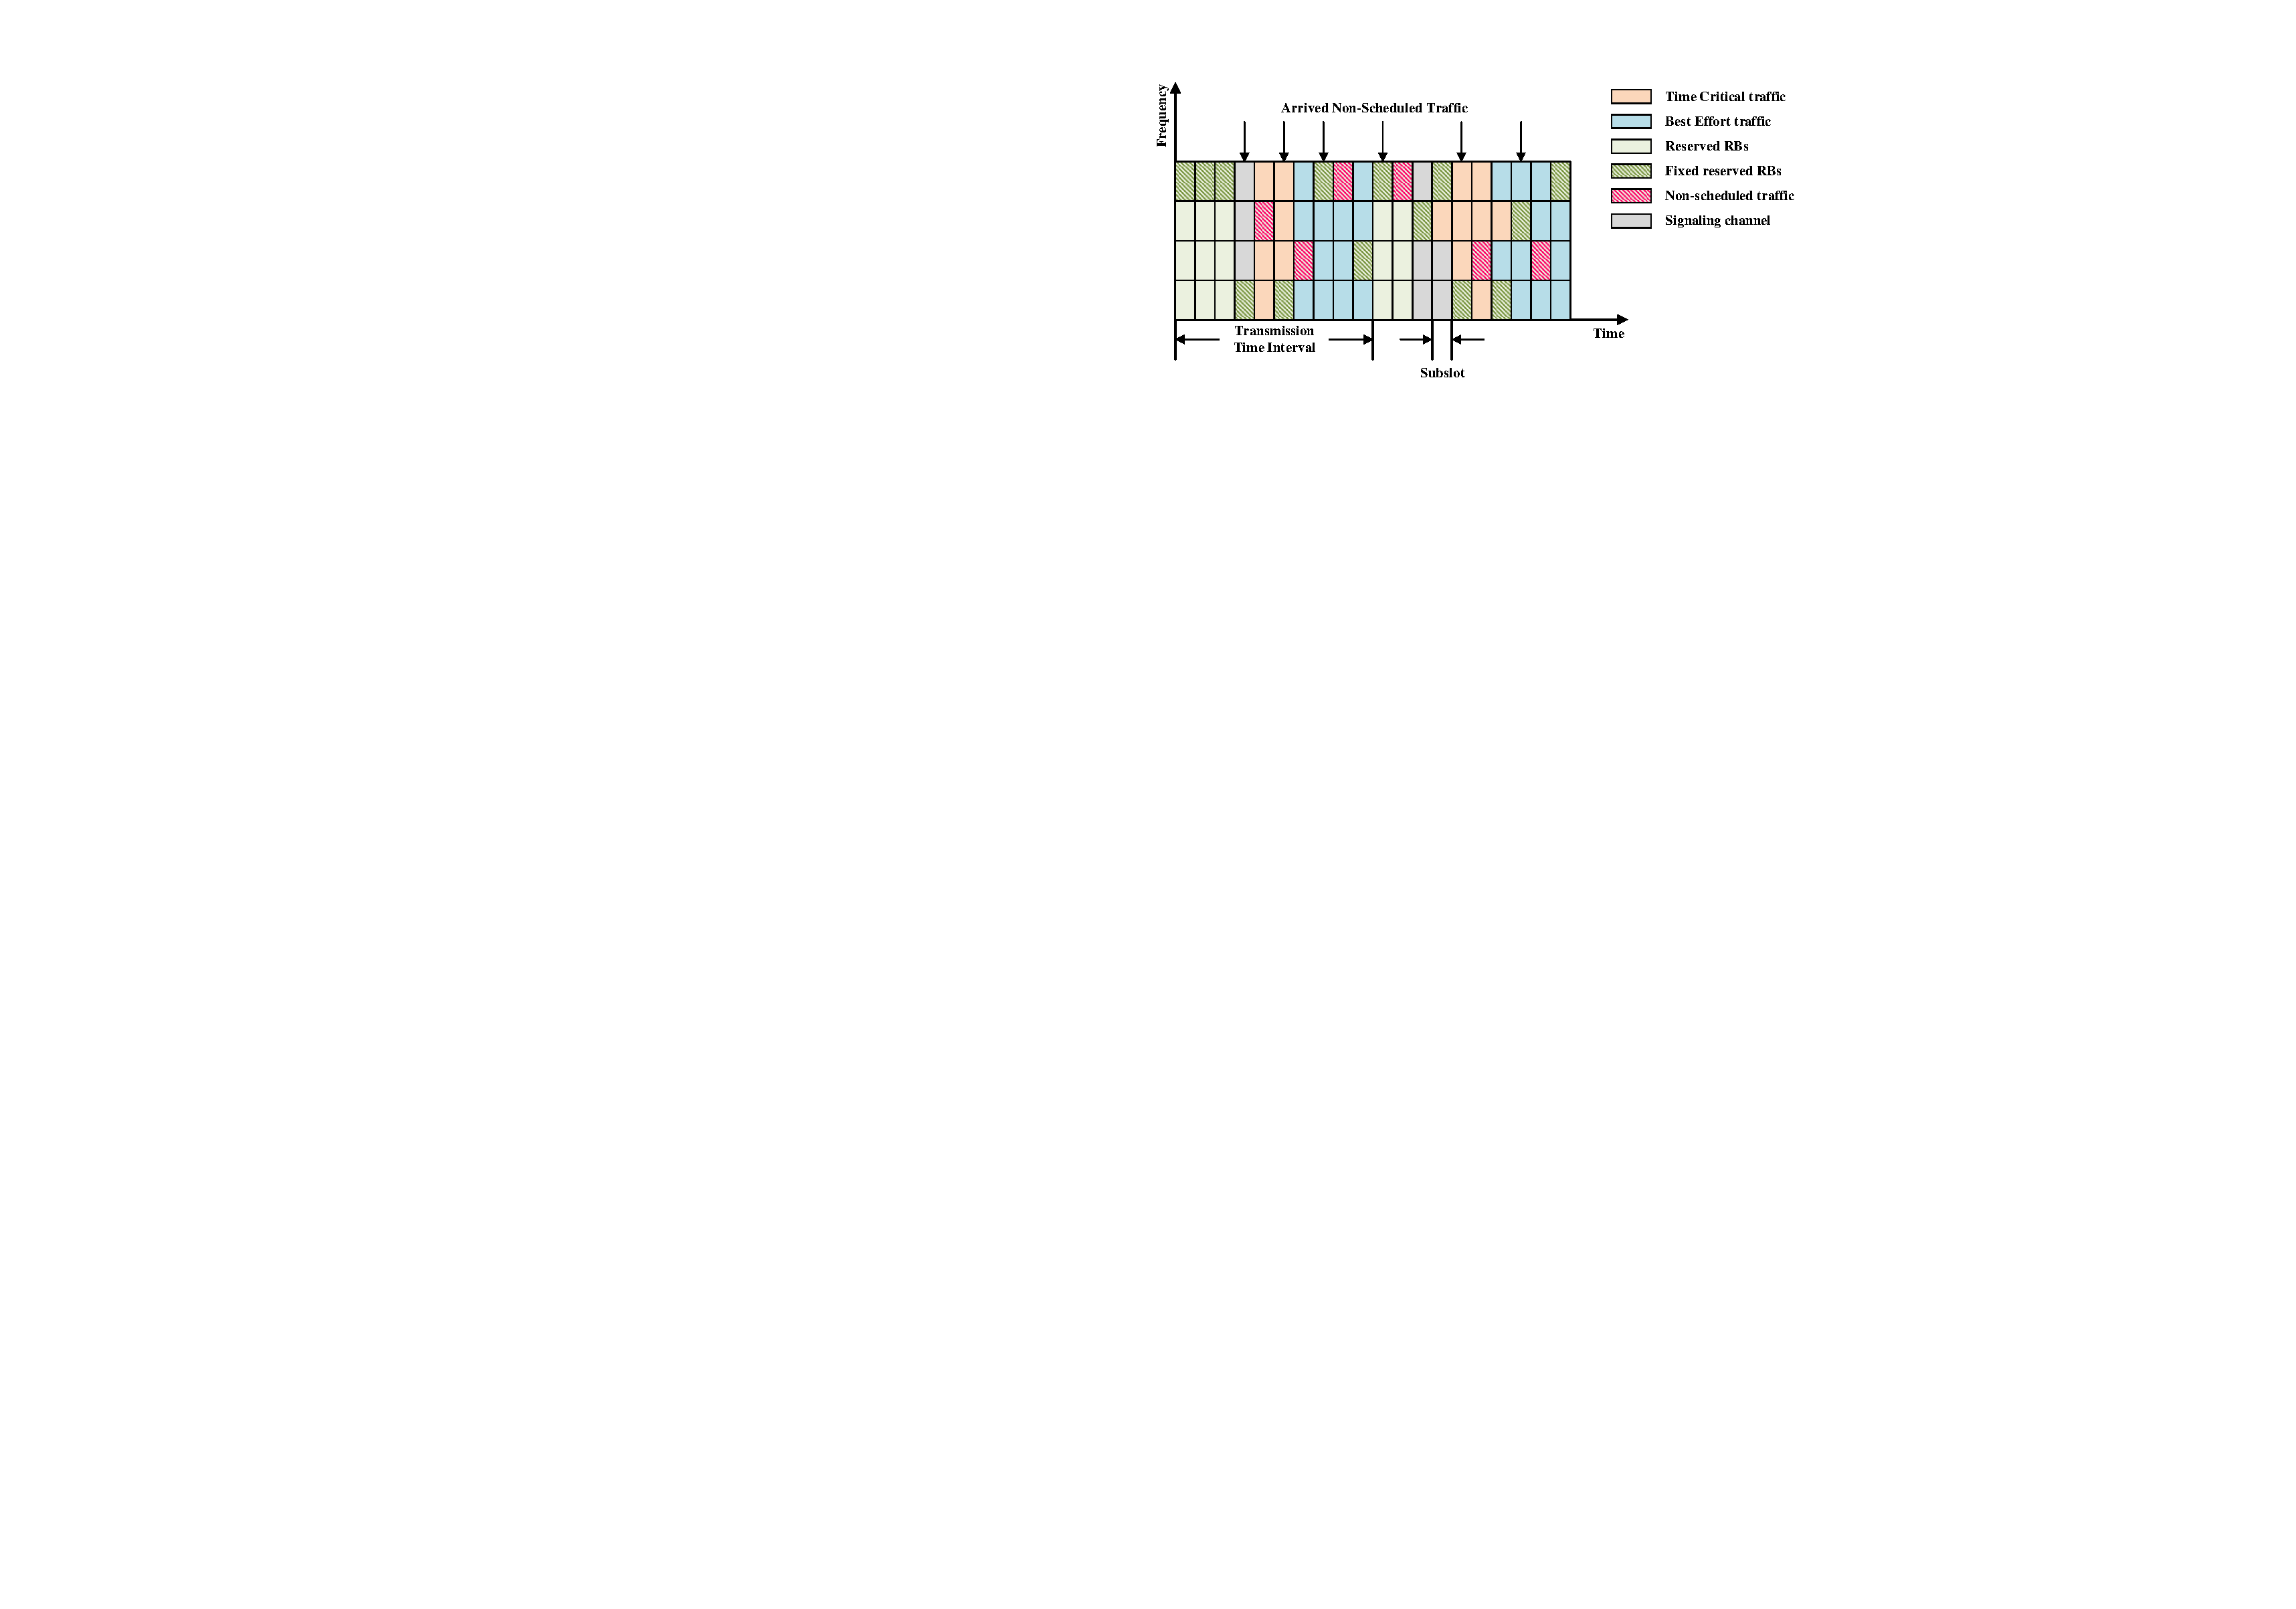
\includegraphics[height=6cm, width=14cm]{RB} 
		\caption{The embedment of multi-priority data in 5G network} 
		\label{fig:RBs}
	\end{figure}
	
	
	%\newpage
	\begin{table}[h]
		\arrayrulecolor{black}
		\caption{\textbf{The Condition of Preemption and Trigger on Fixed Reserved RBs\label{key}}}
		\label{tal:preemption}
		\label{tab1}
		\tabcolsep 40pt %space between two columns.
		\begin{tabular*}{\textwidth}{cccc}
			\toprule
			\bm{$\gamma_{i}=\zeta_{i} \varphi_{i}$} & \textbf{1} & \textbf{0}  \\\hline
			\bm{$\zeta_{i}$} & $r_{\text{brt},i}(t)$ is preempted & $r_{\text{brt},i}(t)$ is not preempted \\
			\bm{$\varphi_{i}$} & $s_{i}(t)$ is triggered & $s_{i}(t)$ is not triggered \\
			\bottomrule
		\end{tabular*}
	\end{table}
	%\footnotetext[1]{test1}
	%\footnotetext[2]{test2}
	
	%\noindent denotes the number of fixed reserved RBs which corresponding sensor is triggered in reservation area, $\zeta(t)=\sum_{i=1}^{\left|\mathcal{R}_{\mathbf{r}}(t)\right| / c} \zeta_{i}$ denotes the number of NS data in reservation area and $\gamma(t)=\sum_{i=1}^{\left|\mathcal{R}_{\mathbf{r}}(t)\right| / C} \gamma_{i}$ denotes the number of reserved RBs that is preempted while its allocated sensor is triggered.
	
	\par Then the number of RBs which are neither triggered nor preempted in the reservation area can be:
	
	\setlength\abovedisplayskip{-13pt}
	\begin{center}
		\begin{equation}
			\left|\mathcal{R}_\mathrm{r}(t)\right|-\left(\left|\mathcal{S}_{\mathrm{e}}(t)\right|+\zeta(t)-\gamma(t)\right)
		\end{equation}
	\end{center}
	\setlength\belowdisplayskip{-8pt}
	
	\noindent where  $\left|\mathcal{S}_{\mathrm{e}}(t)\right|$ is the number of the TC data that embedded in the reservation area. Thus the total number of high priority sensors at TTI $t$, including TC data and embedded NS data, is given by:
	
	\setlength\abovedisplayskip{-13pt}
	\begin{center}
		\begin{equation}
			\begin{aligned}
				\left|\mathcal{S}_{\mathrm{h}}(t)\right| & =\left|\mathcal{R}_\mathrm{r}(t)\right|-\left[\left|\mathcal{R}_\mathrm{r}(t)\right|-\left(\left|\mathcal{S}_{\mathrm{e}}(t)\right|+\zeta(t)-\gamma(t)\right)\right]+\left|\mathcal{S}_{\mathrm{c}}(t)\right|+\left|\mathcal{S}_{\mathrm{b}}(t)\right|-\zeta(t) \\
				& = \left|\mathcal{S}_{\mathrm{e}}(t)\right| +\left|\mathcal{S}_{\mathrm{c}}(t)\right|+\left|\mathcal{S}_{\mathrm{b}}(t)\right| + \varphi(t) - \gamma(t)
			\end{aligned}
		\end{equation}
	\end{center}
	\setlength\belowdisplayskip{-8pt}
	
	\noindent where $\left|\mathcal{S}_{\mathrm{h}}(t)\right|$ is the total number of high priority sensors (TC data and embedded NS data) scheduled at TTI $t$, $\left|\mathcal{S}_{\mathrm{c}}(t)\right|$ and $\left|\mathcal{S}_{\mathrm{b}}(t)\right|$ is the number of sensors generating TC data for dynamic access and the number of sensors generating NS data respectively.
	
	\par Ignore the preemption of NS data, sensors pre-allocated to reserved RBs are scheduled firstly, followed by dynamic access sensors with extra signaling delay, the BE data is scheduled in the end if there are any resources left. The whole transmission process is shown in Figure~\ref{fig:process}. It worth mentioning that we here only focus on the delay of TC data, which is the time difference between the last served TC data and the beginning of the current TTI. The 5G delay can be calculated as follows:
	
	\setlength\abovedisplayskip{-13pt}
	\begin{center}
		\begin{equation}
			T_\text{5G}(t) = \bigg\lceil\frac{\arrowvert \mathcal{R}_{\mathrm{r}}(t) \arrowvert +(\arrowvert S_{\mathrm{c}}(t) \arrowvert + \arrowvert S_{\mathrm{b}}(t) \arrowvert -(\zeta(t) - \gamma(t)))(1+\delta) }{|C|} \bigg\rceil*T_\text{RB}
		\end{equation}
	\end{center}
	\setlength\belowdisplayskip{-8pt}
	
	\noindent where $T_\text{RB}$ is the time duration corresponding to one RB, $\delta$ is the proportion of signaling in the overall transmission and $\lceil*\rceil$ represents the smallest integer which $*$ is less than or equal to.
	It can be seen from Figure~\ref{fig:RBs} that if the last TC sensor is left in the last column alone, the 5G delay will be extended for one $T_\text{RB}$.
	
	
	\begin{figure}[h] 
		\centering 
		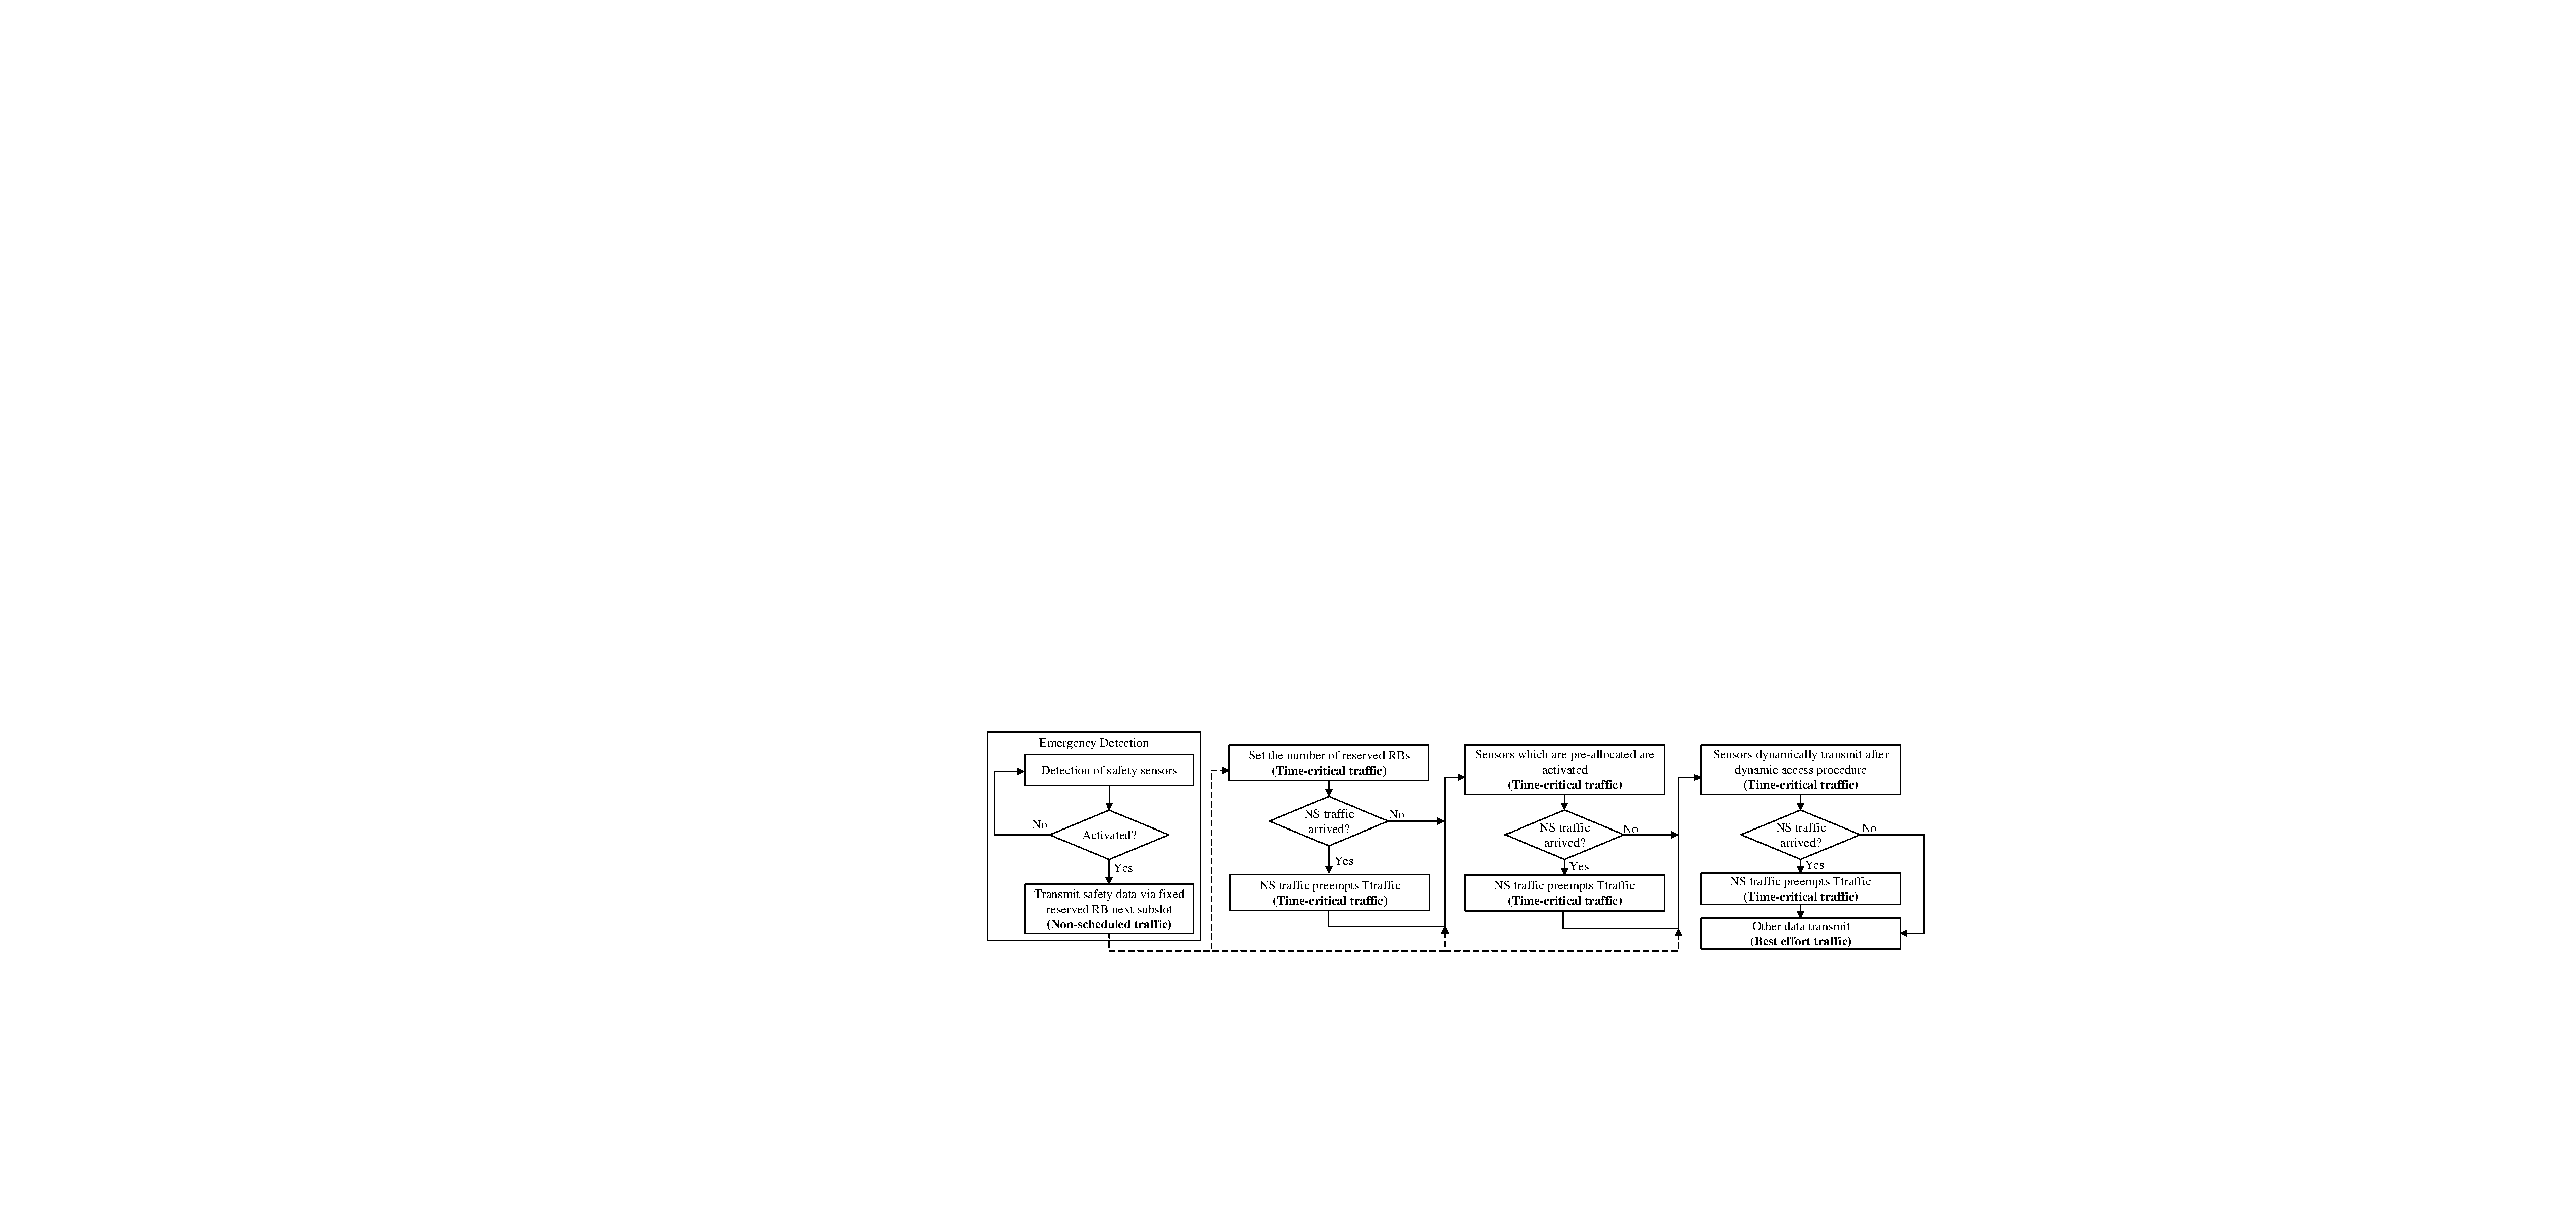
\includegraphics[height=4cm, width=16.2cm]{wireless_trans_mech} 
		\caption{The process of Multi-priority data Transmission with Preemption Considered} 
		\label{fig:process}
	\end{figure}
	
	
	
	
	\begin{comment}
	\begin{algorithm}[H]
	\SetAlgoLined
	\KwIn{Access samples at last TTI $\bm{x}(t)=\{x_{1}(t), x_{2}(t), ...\}$,\\ \qquad\quad\, History access samples $H_{n} = \{h_{1}, h_{2}, ..., h_{n}\}$}
	\KwOut{Predictive select sensors sets $\bm{y}(t) = \{y_{1}(t), y_{2}(t), ...\}$} 
	\SetKwInput{Initialization}{Initialization}
	\Initialization{Trigger time set $T = \varnothing$, $\bm{y}(t) = \varnothing$}
	\SetKwInput{KwIn}{Input}
	\For{j = \rm1,2,3,…}{
	$T += h_{j}$		
	}
	\For{i = \rm1,2,3,…}{
	\uIf {$T(j) \leqslant \beta$ and $y_{i}(t) \not\in \bm{x}(t)$} {
	$\mathbb{P}(y_{i}(t), \bm{x}(t)) = \mathbb{P}_{\chi^{2}}(y_{i}(t), \bm{x}(t))$
	} 
	\ElseIf {$T(j) > \beta$ and $y_{i}(t) \not\in \bm{x}(t)$} {
	$\mathbb{P}(y_{i}(t), \bm{x}(t)) = \mathbb{P}_{\mathrm{MI}}(y_{i}(t), \bm{x}(t))$
	}
	\If{$\Pi_\text{sel}$}{
	$\bm{y}(t) = \bm{y}(t)\cup \lbrace y_{i}(t)\rbrace $
	}
	}
	\caption{Sensor Selection Algorithm(SSA)}
	\end{algorithm}
	\end{comment}
	
	
	\subsection{Data Injection Model of TSN Gateways}  
	As mentioned in Section~\ref{sec:Overview of HTSN}, there are several queues of each port of TSN gateways, which have different priorities while transmitting via TSN. The coordination of TAS and GCL can make sure the data forwarded in TSN can be deterministically delivered within its time demand while keeping its priority.
	
	\par PSFP mechanism proposed by IEEE 802.1Qci points out that each data arrived owns a priority number, named IPV, to be a reference to transmit data heterogeneously in TSN. In more detail, every data will be assigned a Gate ID to match its IPV number, where each Gate ID represents a TSN sending queue, so the data with different IPV will be injected into different TSN queues. It can be seen that the key to deciding which queue to inject is the value of IPV, so we propose a data injection mechanism of TSN gateways based on IPV to offset the time deviation such as jitters caused by 5G network. Thus, the TSN delay is reduced according to the 5G network delay. Note that the data with lower IPV number has higher priority.
	
	\par Outlined in Figure~\ref{fig:Injection Policy}, the data from the 5G network will be firstly gathered into a frame pool, where data generated within a TTI is classified into different priorities (refered to as IPV numbers) according to its 5G delay, and then it is injected into different TSN queue dynamically.
	
	\begin{figure}[t] 
		\centering 
		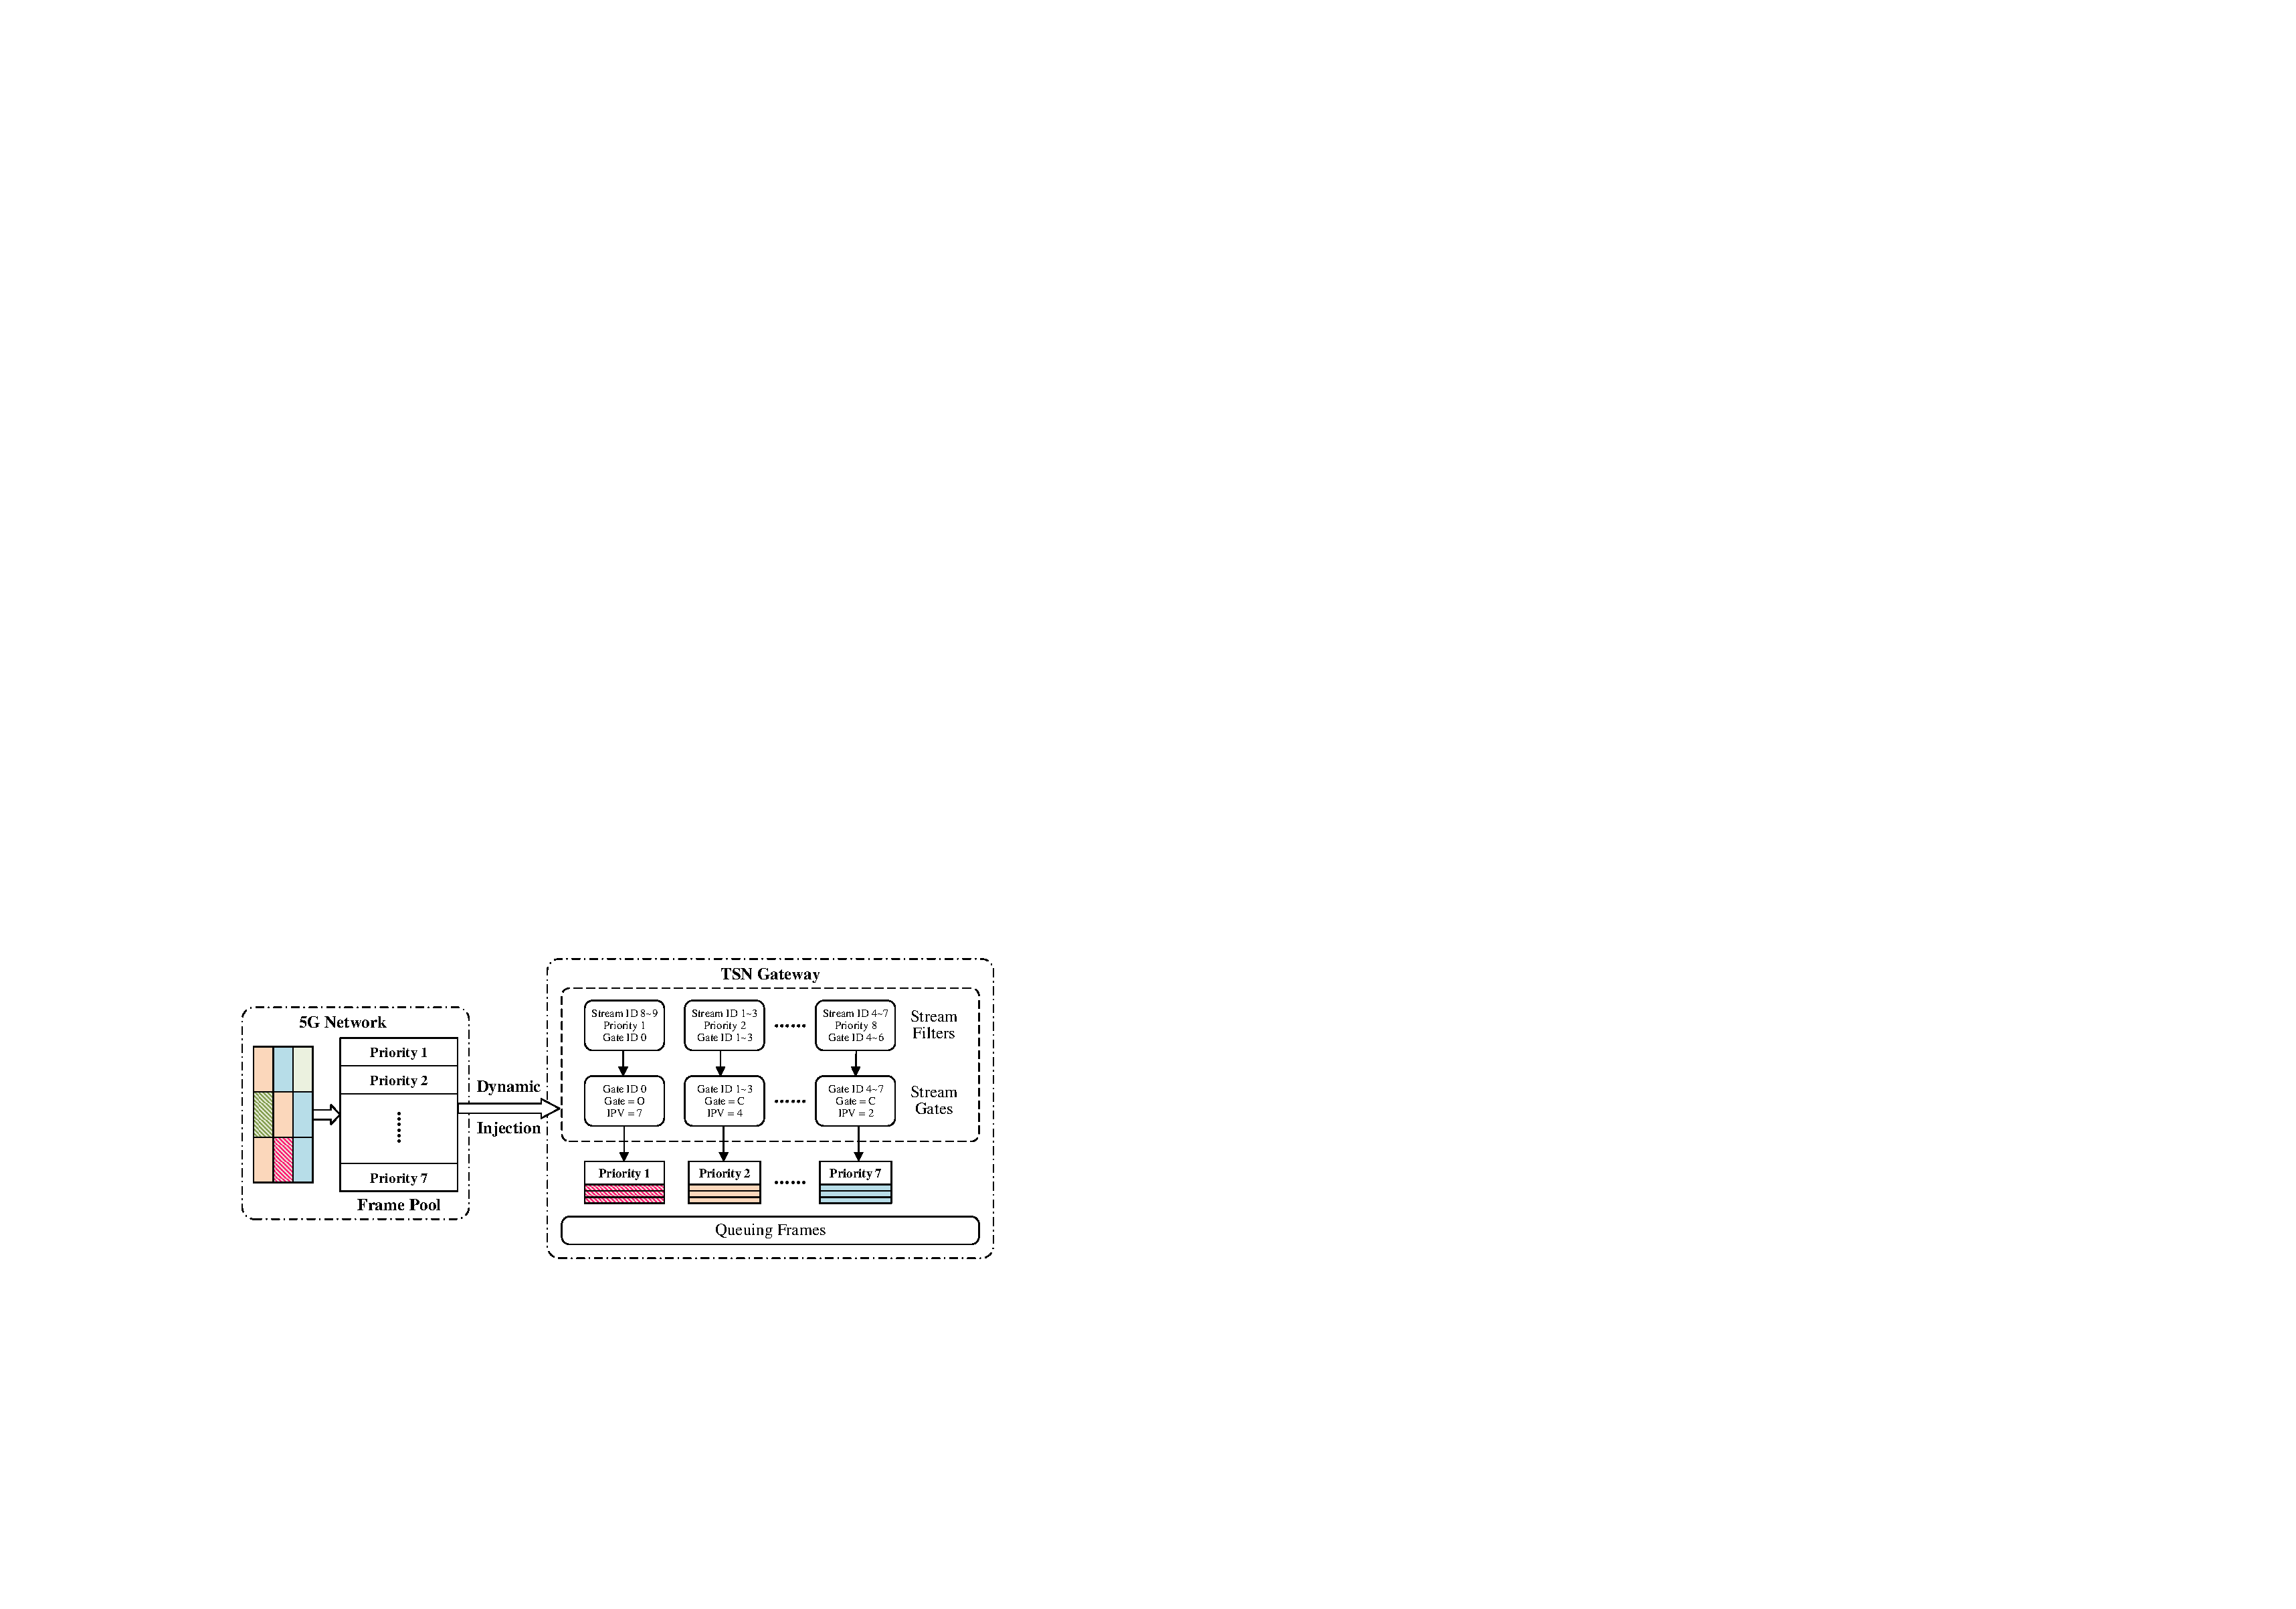
\includegraphics[height=5.5cm, width=14cm]{Injection} 
		\caption{Injection Policy of TSN Queue Based on PSFP} 
		\label{fig:Injection Policy}
	\end{figure}
	
	
	
	\par First, we divide the forwarding delay of TC data via TSN into $x$ parts:
	
	\setlength\abovedisplayskip{-16pt}
	\begin{center}
		\begin{equation}
			\Delta=\frac{T_{\text{TSN}}^{\text{max}}-T_{\text{TSN}}^{\text{min}}}{x}, x=1,2, \ldots \ldots
		\end{equation}
	\end{center}
	\setlength\belowdisplayskip{-8pt}
	
	\vspace{-6pt}
	\noindent where $T_{\text{TSN}}^{\text{max}}$ and $T_{\text{TSN}}^{\text{min}}$ denotes the maximum and the minimum forwarding delay through TSN respectively, $x$ is the number of queues of a TSN port, which is usually eight.
	
	\par Thus we can get the forwarding deadline of each queue as follows:
	
	\setlength\abovedisplayskip{-16pt}
	\begin{center}
		\begin{equation}
			\Lambda\left(Q(t)\right)=T_{\text{TSN}}^{\text{min}}+Q(t) * \Delta,  Q(t)=1,2, \ldots, x
		\end{equation}
	\end{center}
	\setlength\belowdisplayskip{-8pt}
	
	\vspace{-6pt}
	\noindent where $Q(t)$ is the IPV number of arriving data from 5G at TTI $t$. Therefore we get the forwarding delay function of $Q(t)$, which can be used to calculate the delay of TSN and get the number of $Q(t)$ in reverse.
	
	\par  The TSN delay with different queue is calculated by:
	
	\setlength\abovedisplayskip{-16pt}
	\begin{center}
		\begin{equation}
			T_\text{TSN}(t)=H\bigg\lceil\frac{\left|\mathcal{S}_{\mathrm{h}}(t)\right| * D * \Lambda\left(Q(t)\right)}{\theta_\text{low} T_{\text{cyc}}}\bigg\rceil T_{\mathrm{cyc}}
		\end{equation}
	\end{center}
	\setlength\belowdisplayskip{-8pt}
	
	\vspace{-6pt}
	\noindent where $\left|\mathcal{S}_{\mathrm{h}}(t)\right|$ has been given in Section~\ref{sssec:preemption}, $H$ is the number of hops within TSN with fixed beginning and terminal, $D$ is the fixed amount of data that one RB transmit, $T_{\mathrm{cyc}}$ is the forwarding cycle of TSN gateways and $\theta_\text{low}$ is the lowest data rate of TSN.
	
	\par Based on the TSN delay we get above, the value of $Q(t)$ is obtained by $\Lambda\left(Q(t)\right)$ as follows:
	
	\setlength\abovedisplayskip{-16pt}
	\begin{center}
		\begin{equation}
			Q(t)=\arg \min _{1 \leq Q(t) \leq x}\left(T_\text{TSN}(t)-\left(T_\text{ddl}(t)-T_\text{5G}(t)\right)\right)
		\end{equation}
	\end{center}
	\setlength\belowdisplayskip{-8pt}
	
	\vspace{-6pt}
	\noindent where $T_\text{ddl}(t)$ is the delay demand of TC data arrived at TTI $t$, and $T_\text{5G}(t)$ is the transmission delay through previous 5G network.
	
	
	
	\par Thus the whole transmission delay under HTSN at TTI $t$ is given by:
	
	\setlength\abovedisplayskip{-16pt}
	\begin{center}
		\begin{equation}
			T_\text{E2E}\left(T_\text{5G}(t), T_\text{TSN}(t)\right)=T_\text{5G}(t)+T_\text{TSN}\left(Q(t), \mathcal{F}\left(T_\text{5G}(t)\right)\right)
		\end{equation}
	\end{center}
	\setlength\belowdisplayskip{-8pt}
	
	\vspace{-6pt}
	\par {\color{blue}Obviously, the delay of 5G network $T_\text{5G}(t-1)$ and the delay of TSN $T_\text{TSN}(t-1)$ is coupling and interact with each other as shown in Figure \ref{fig:flow}. In particular, we first take the cumulative transmission delay $\sum_{m=1}^{t-2} T(m)$ as the prior information to obtaine the number of reserved RBs $\mathcal{R}_{\mathrm{r}}(t-1)$ at TTI $t-1$. Then according to the 5G delay calculated by $\mathcal{R}_{\mathrm{r}}(t-1)$ and the couping relationship between 5G delay and TSN delay, we can get the IPV number of TC data based on the data injection model above. Finally, on the basis of the newly get $T_\text{5G}(t-1)$ and $T_\text{TSN}(t-1)$, we can get the whole transmission delay $T_\text{E2E}(t-1)$ under HTSN at TTI $t-1$, whereby it can be added into the cumulative transmission delay $\sum_{m=1}^{t-1} T(m)$ and become the prior information of TC data in TTI $t$.}
	
	\begin{figure}[h] 
		\centering 
		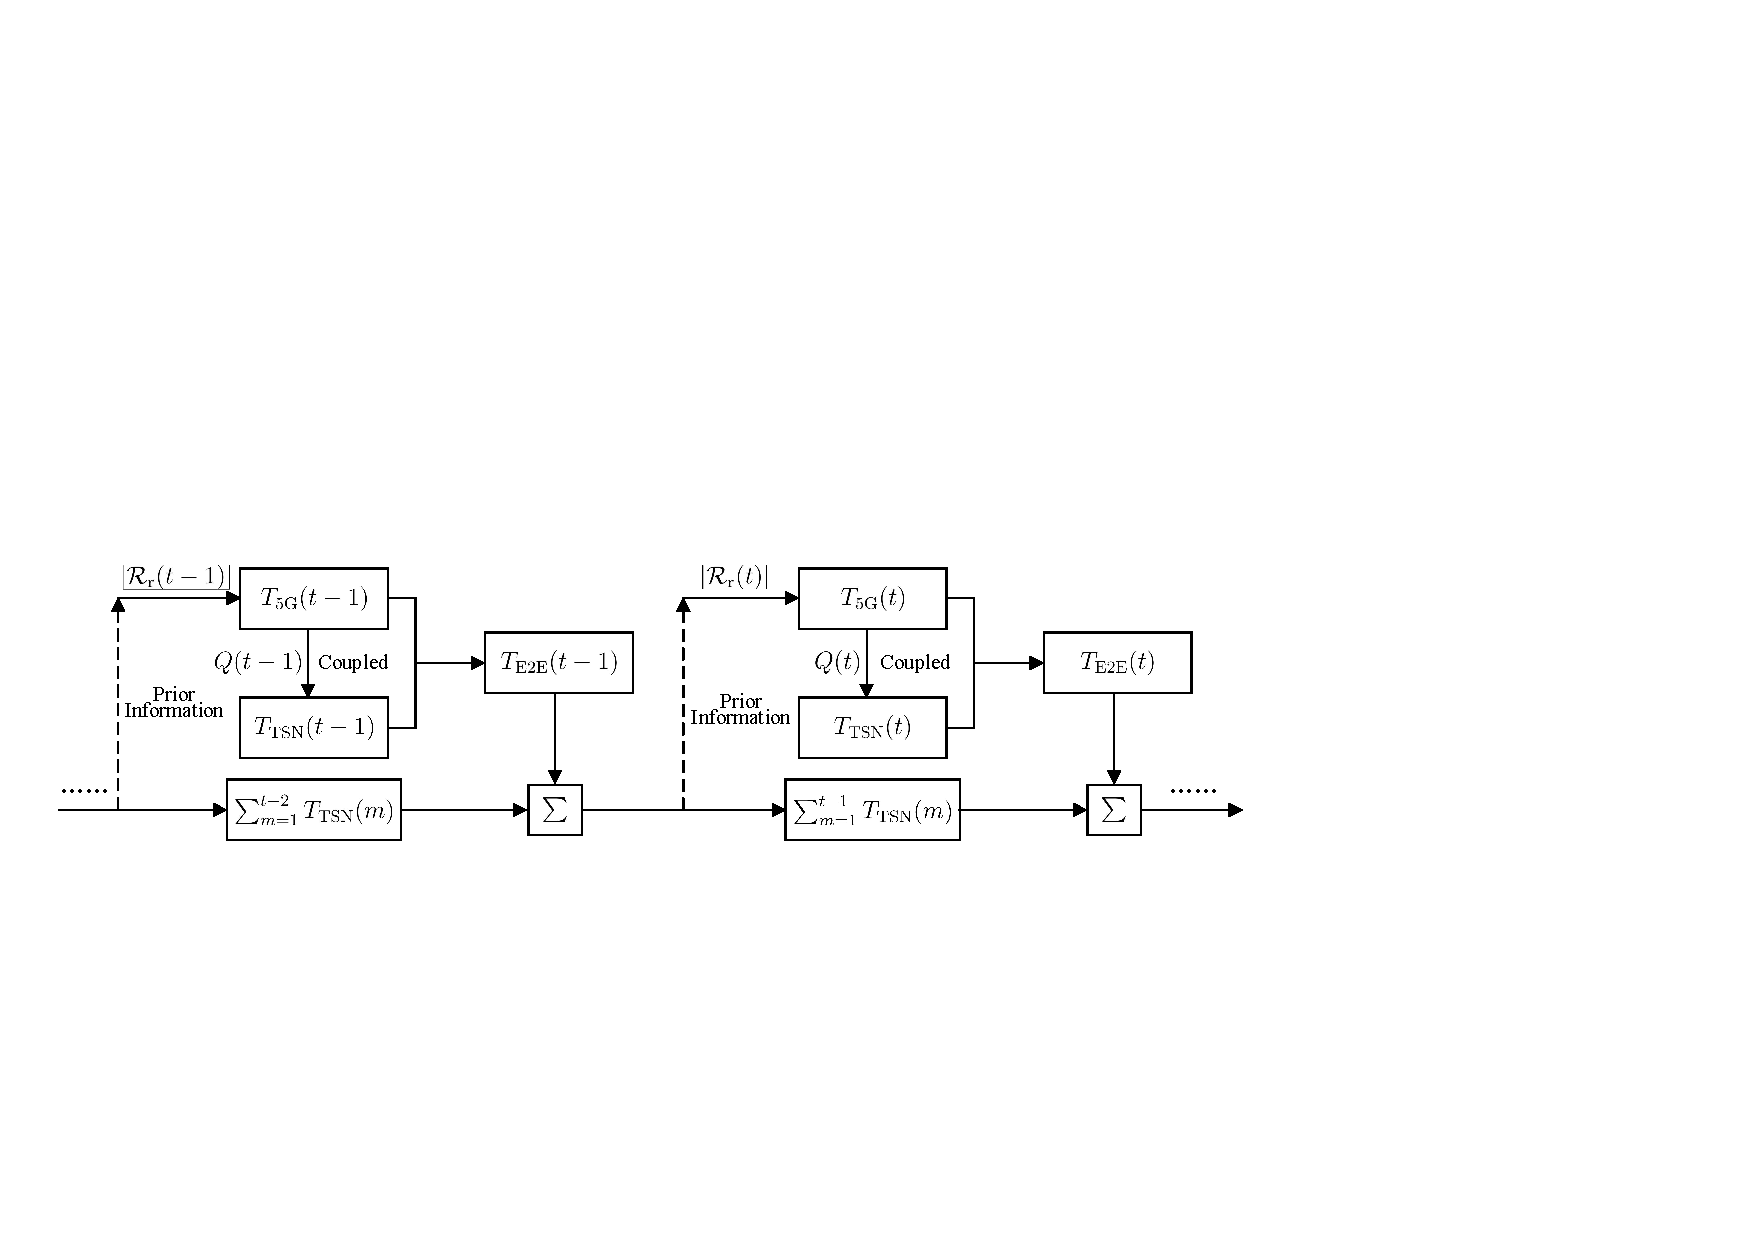
\includegraphics[height=3.6cm, width=15.5cm]{flow} 
		\caption{The flow of TC data under HTSN} 
		\label{fig:flow}
	\end{figure}
	
	\subsection{Risk-sensitive Utility Formulation} 
	\label{ssec:risk-sensitive problem}
	Considering the unreliability of 5G network, the higher-order quantity of wireless delay should be involved in the optimal problem as mentioned in Section~\ref{sec:introduction}. In this regard, we apply entropic risk measure $\frac{1}{\rho} \ln \left(\mathbb{E}\left[\exp \left(\rho T\right)\right]\right)$ and formulate a risk-sensitive minimization utility function of the whole transmission delay under HTSN with  as follows\cite{bennis2018ultrareliable}:
	
	
	\setlength\abovedisplayskip{-16pt}
	\begin{center}
		\begin{equation}
			\begin{aligned}
				\bm{\mathcal{P}1:} \underset{\left\{\left|\mathcal{R}_\mathrm{r}(t)\right|, Q(t)\right\}}{\mathrm{min}} &\frac{1}{\rho} \ln (\mathbb{E}[\exp (\rho \sum_{m=1}^{t-1} T(m))]) \\
				\text { s.t. } &\left|\mathcal{R}_\mathrm{r}(t)\right| \leq\left| \Pi^\text{sel} \right|  \\
				&1 \leq Q(t) \leq 8
			\end{aligned}
		\end{equation}
	\end{center}
	\setlength\belowdisplayskip{-8pt}
	
	\vspace{-6pt}
	\noindent where $\mathbb{E}[*]$ is the expectation operator, $\left| \Pi^\text{sel} \right|$ represents the number of predictive selected candidate sensors which is described in detail in Section \ref{sec:selection}.
	
	\par The entropic risk measure $\frac{1}{\rho} \ln \left(\mathbb{E}\left[\exp \left(\rho \mathcal{T}\right)\right]\right)$ can be expanded out as $\frac{1}{\rho} \ln (\mathbb{E}[\exp (\rho \mathcal{T})])=\mathbb{E}[\mathcal{T}]+\frac{\rho}{2 !} \operatorname{Var}(\mathcal{T})+\frac{\rho^{2}}{3 !} \mathbb{E}\left[(\mathcal{T}-\mathbb{E}[\mathcal{T}])^{3}\right]+...$, where $\mathcal{T}$ denotes the cumulative time $\sum_{m=1}^{t-1} T(m)$. It is obvious that the optimal object takes into account the variance $\operatorname{Var}(\mathcal{T})$ and the third central moment $\mathbb{E}\left[(\mathcal{T}-\mathbb{E}[\mathcal{T}])^{3}\right]$ of $\mathcal{T}$. Note that the skewness of $\mathcal{T}$ equals to $\mathbb{E}\left[(\mathcal{T}-\mathbb{E}[\mathcal{T}])^{3}\right] / \operatorname{Var}((\mathcal{T}))^{\frac{3}{2}}$. In other words, we formulate the optimization problem in the view of the mean, varience, skewness and other high-order quantity of the cumulate time $\sum_{m=1}^{t-1} T(m)$. Additionally, the parameter $\rho > 0$ reflects the weight of high-order statistics. 
	
	\par Due to the function $\frac{1}{\rho} \ln \left(*\right)$ is monotonically increasing, we remove it and focus on an equivalent utility problem as follows:
	
	\setlength\abovedisplayskip{-16pt}
	\begin{center}
		\begin{equation}
			\label{p2}
			\begin{aligned}
				\bm{\mathcal{P}2:} \underset{\left\{\left|\mathcal{R}_\mathrm{r}(t)\right|, Q(t)\right\}}{\mathrm{min}} &\mathbb{E}[\exp (\rho \sum_{m=1}^{t-1} T(m))] \\
				\text { s.t. } &\left|\mathcal{R}_\mathrm{r}(t)\right| \leq\left| \Pi^\text{sel} \right|  \\
				&1 \leq Q(t) \leq 8
			\end{aligned}
		\end{equation}
	\end{center}
	\setlength\belowdisplayskip{-8pt}
	
	\vspace{-5pt}
	\noindent which can be expanded by Maclaurin series expansion analogously, i.e., $\mathbb{E}[\exp (\rho \mathcal{T})] = 1 + \rho \mathbb{E}[\mathcal{T}] + \frac{\rho^2}{2!} \mathbb{E}[\mathcal{T}^2] + \frac{\rho^3}{3!} \mathbb{E}[\mathcal{T}^3]$ for $\mathcal{T} = \sum_{m=1}^{t-1} T(m)$.
	
	\par It is challenging to solve the minimization problem because of TSN's dynamic network state and the unknown environmental factors of each gateway. Thus, we leverage the principles of multi-armed bandits(MAB) in reinforcement learning to optimize the long-term transmission delay in a decentralized manner.
	
	\section{Risk-sensitive Learning Strategy for Predictive Scheduling}
	\label{learning} 
	For the minimization problem we formulated above, a risk-sensitive learning (RSL) strategy is proposed to solve the problem in a static stage and a dynamic stage. The static stage attempts to improve the prediction precision and constrain the number of reserved RBs by selecting sensors through the access history. Then the total delay and the long delay tail of $T_\text{E2E}$ are considered in the dynamic stage based on the gradient multi-armed bandits (GMAB) scheme.
	
	
	\subsection{Static Stage: Sensor Selection Algorithm Based on Naive Bayesian Model}~{}
	\label{sec:selection}
	\par As discussed above, the main task of the static stage is to select the most correlated sensors to compose the reservation candidates set. Obviously, the utilization of reserved RBs is determined by whether assigned sensors trigger. So a high prediction precision is necessary to reduce 5G transmission delay. Besides, a salient feature of industrial automation is that the trigger of one event-triggered MTC device may increase the probability that other devices in the vicinity also generate data in quick succession\cite{shafiq2013large,li2018predictive}. Based on this, calculate the correlation between sensors at two adjacent TTIs is the key to predictive select sensors to be reserved. Here we don't care about the relationship between sensors but only concern the correlation between their trigger. In the literature\cite{li2018predictive}, we apply the Naive Bayesian model to learn the correlation of sensors since it simplifies the assumption of conditional independence,.
	
	
	\par Let $\bm{x}(t)=\{x_{1}(t), x_{2}(t), ...\}$ denotes the set of sensors triggered at TTI $t-1$, we select sensors to make up the reservation candidates set $\bm{y}(t) = \{y_{1}(t), y_{2}(t), ...\}(\bm{x}(t) \cap \bm{y}(t) = \varnothing)$, which may be triggered at the TTI $t$ with a high probability. Note that the scale of $\bm{y}(t)$ lies on the threshold $\alpha$ we set and is not related to the scale of $\bm{x}(t)$.
	
	\par In order to explore the correlation between sensors, the access history is used to get the trigger probability of sensor $y_{i}(t)$ as $\bm{\mathbb{P}}(y_{i}(t)) (y_{i}(t) \in \mathcal{S})$, then three metrics are used to measure the correlation between the set $\bm{x}(t)$ and the sensor $y_{i}(t)$ as follows\cite{sanasam2010feature}:
	
	\par 1) \textbf{Conditional probability}: Conditional probability at TTI $t$ is the probability that sensors out of $\bm{x}(t)$ will trigger after any sensors in $\bm{x}(t)$ that has been triggered, which can be obtained by:
	
	\setlength\abovedisplayskip{-15pt}
	\begin{center}
		\begin{equation}
			\mathbb{P}_{\mathrm{C}}(y_{i}(t),  \bm{x}(t))= \mathbb{P}(y_{i}(t) \mid x_{j}(t))= \sum_{x_{j}(t)\in \bm{x}(t)} \frac{\mathbb{P}(y_{i}(t), x_{j}(t))}{\mathbb{P}(x_{j}(t))}
		\end{equation}
	\end{center}
	\setlength\belowdisplayskip{-8pt}
	
	\vspace{-6pt}
	\noindent where $\mathbb{P}(y_{i}(t), x_{j}(t))$ is the joint probability of $y_{i}(t)$ and $x_{j}(t)$, and it is calculated as $\mathbb{P}(y_{i}(t), x_{j}(t)) = \mathbb{P}(y_{i}(t) \mid x_{j}(t)) * \mathbb{P}(x_{j}(t))$.
	
	\par 2) \textbf{Mutual information (MI)}: As described in information theory, MI can measure the development of the trigger probability of $y_{i}(t)$ after $\bm{x}(t)$ is triggered, which is given by:
	
	\setlength\abovedisplayskip{-15pt}
	\begin{center}
		\begin{equation}
			\mathbb{P}_{\mathrm{MI}}(y_{i}(t), \bm{x}(t))= \sum_{x_{j}(t)\in \bm{x}(t)} \mathbb{P}(y_{i}(t), x_{j}(t)) \log _{2} \frac{\mathbb{P}(y_{i}(t), x_{j}(t))}{\mathbb{P}(y_{i}(t)) \mathbb{P}(x_{j}(t))}
		\end{equation}
	\end{center}
	\setlength\belowdisplayskip{-8pt}
	
	\vspace{-6pt}
	\noindent where $\mathbb{P}(y_{i}(t), x_{j}(t)) = \mathbb{P}_{\mathrm{C}}(y_{i}(t), x_{j}(t)) * \mathbb{P}(x_{j}(t))$.
	
	\par 3) \textbf{Chi-square s ($\chi^{2}$)}: Chi-square ($\chi^{2}$) text is a suitable way to estimate the relevance of two sensors by comparing $\mathbb{P}(y_{i}(t), x_{j}(t))$ and $\mathbb{P}(y_{i}(t)) * \mathbb{P}(x_{j}(t))$, so to judge whether these two sensors are dependent, we use $\chi^{2}$ test metric as below:
	
	\setlength\abovedisplayskip{-16pt}
	\begin{center}
		\begin{equation}
			\mathbb{P}_{\mathrm{\chi^{2}}}(y_{i}(t), \bm{x}(t))= \sum_{x_{j}(t)\in \bm{x}(t)} \frac{(\mathbb{P}(y_{i}(t), x_{j}(t)) - \mathbb{P}(y_{i}(t)) * \mathbb{P}(x_{j}(t)))^{2}}{\mathbb{P}(y_{i}(t)) * \mathbb{P}(x_{j}(t))}
		\end{equation}
	\end{center}
	\setlength\belowdisplayskip{-8pt}
	
	
	%
	\vspace{-6pt}
	\par The aim of these three metrics is to evaluate the correlation between $y_{i}(t)$ and $\bm{x}(t)$. Thus we can select the most relevant sensors to $\bm{x}(t)$ to be reserved predictively at TTI $t$ for higher resource utilization and lower transmission delay. Thus we use a policy $\Pi^\text{sel}=\{\pi_{1}, \pi_{2}, \dots\}$ to choose which sensor to reserve as:
	
	\setlength\abovedisplayskip{-16pt}
	\begin{center}
		\begin{equation}
			\label{pi}
			\pi_{i}=\left\{\begin{array}{ll}1, & \text { if } \mathbb{P}(y_{i}(t), \bm{x}(t)) \geq \alpha \\0, & \text { otherwise }
			\end{array}\right.
		\end{equation}
	\end{center}
	\setlength\belowdisplayskip{-8pt}
	
	\par {\color{blue}As we can see from the equation (\ref{pi}), the number of the reserved RBs depends on the threshold $\alpha$ we set, since $\pi_{i}=1$ when $\mathbb{P}(y_{i}(t), \bm{x}(t)) \geq \alpha$. In fact, there exists a trade-off of the number of reserved RBs $\left|\mathcal{R}_\mathrm{r}(t)\right|$ for the following reasons. If $\left|\mathcal{R}_\mathrm{r}(t)\right|$ is too small, most of the sensors still need to access the 5G network dynamically with a high handshaking cost, which may violate the time demand of NS data and TC data. On the other hand, if $\left|\mathcal{R}_\mathrm{r}(t)\right|$ is too big but the prediction precision cannot be guaranteed, the time-frequency resources left will be insufficient for for dynamic access sensors. Besides, the reserved resources will also be wasted a lot. Therefore, $\alpha$ is a critical factor to balance this trade-off.}
	
	%\vspace{-6pt}
	\par Form\cite{li2018predictive} we know that sensors with lower trigger frequency will obtain a higher ranking in the $\chi^{2}$ test than in the MI. Based on this, we propose a sensor selection algorithm that is outlined in Algorithm 2 for good practicability. Note that the $i$-th elements of $n$ history access samples set $\bm{H_{n}}$ is boolean set $\bm{h_{i}}$. And $\beta$ is the threshold of trigger time used to select a metric.
	
	\begin{algorithm}
		%\floatname{algorithm}{Algorithm}%¸ü¸ÄË㷨ǰ׺Ãû³Æ
		\renewcommand{\algorithmicrequire}{\textbf{Input:}}%¸ü¸ÄÊäÈëÃû³Æ
		\renewcommand{\algorithmicensure}{\textbf{Output:}}%¸ü¸ÄÊä³öÃû³Æ
		\footnotesize
		\caption{Sensor Selection Algorithm(SSA)}
		\label{alg1}
		{\fontsize{10}{12}\selectfont
			\begin{algorithmic}[1]
				\REQUIRE Access samples at last TTI $\bm{x}(t)=\{x_{1}(t), x_{2}(t), ...\}$;\\ \qquad  History access samples $\bm{H_{n}} = \{\bm{h_{1}, h_{2}, ..., h_{n}}\}$;\\ \qquad Trigger time set $T = \{0\} $ with length $n$, $\bm{y}(t) = \varnothing$;
				\ENSURE Predictive select sensors sets $\bm{y}(t) = \{y_{1}(t), y_{2}(t), ...\}$;
				\WHILE{$j \leq n$}
				\STATE $T = T + h_{j}$
				\ENDWHILE
				\WHILE{$i \leq |\bm{x}(t)|$}
				\IF{$T(i) \leqslant \beta$ and $y_{i}(t) \not\in \bm{x}(t)$}
				\STATE $\mathbb{P}(y_{i}(t), \bm{x}(t)) = \mathbb{P}_{\chi^{2}}(y_{i}(t), \bm{x}(t))$;
				\ELSE[$T(i) > \beta$ and $y_{i}(t) \not\in \bm{x}(t)$]
				\STATE $\mathbb{P}(y_{i}(t), \bm{x}(t)) = \mathbb{P}_{\mathrm{MI}}(y_{i}(t), \bm{x}(t))$;
				\ENDIF
				\IF{$\Pi_\text{sel}$}
				\STATE $\bm{y}(t) = \bm{y}(t)\cup \lbrace y_{i}(t)\rbrace $;
				\ENDIF
				\ENDWHILE
			\end{algorithmic}
		}
	\end{algorithm}
	
	\par In static stage, we use three different metrics to measure the correlation of sensors according to different scenarios, which can improve the precision of sensor selection, and then reduce the delay of 5G network by multi-priority scheduling based on SPS while considering preemption.
	
	
	\subsection{Dynamic Stage: RSL Algorithm Based on GMAB}
	As mentioned in Section~\ref{sec:selection}, the number of reserved RBs $\left|\mathcal{R}_\mathrm{r}(t)\right|$ brings a trade-off. There are three parameters that are influenced by this trade-off such as the 5G delay, the IPV number of data when it is injected into TSN gateway, and the whole transmission delay under HTSN. Each TSN gateway needs to make decisions based on a limited state information every TTI to find out the optimal policy to dynamic reserve RBs and inject data into its sending queue while guaranteeing the time demand as well. This predictive pre-allocation problem with no prior knowledge is skin to the famous multi-armed bandits' problem\cite{li2018predictive,arora2011sequential,xu2017data}, which also concerns the balance of multiple arms' exploration and exploitation to gain the long-term rewards via trying to choose different arms.
	
	\par We here leverage the GMAB tool to solve the predefined problem since it only focuses on the relative preferences between actions rather than the value of the action itself. In particular, each TSN gateway acts as an agent that selects an action to maximize the long-term rewards. The action set is defined as $k=\left(k_{1}, k_{2}, \ldots, k_{\left|k\right|}\right)$, where $k_{i}=\left(\left|\mathcal{R}_{\mathrm{r}}(i)\right|, Q_{i}\right)$ denotes the corresponding action of the $i$-th arm. The policy gateway made at TTI $t$ is given by $\varpi(t)=\{\varpi_{1}(t), \varpi_{2}(t), \ldots, \varpi_{\left|k\right|}(t)\}$, which means the agent chooses the $i$-th arm with probability $\varpi_{i}(t)$ at TTI $t$. Here we denote the long-term delay in (\ref{p2}) as a utility function $U(t) =-\exp (\rho \sum_{m=1}^{t-1} T(m))$. The main step of GMAB algorithm are outlined as follows:
	
	
	\begin{itemize}[itemsep= 15 pt,topsep = -1.5 pt]
		\item[(1)]
		Each TSN gateway is given an initial policy: $\varpi(0)=\{\varpi(0,1), \varpi(0,2), \ldots, \varpi(0,\left|k\right|)\}$, and the preference function $H(t,k_{i})$ of each action is the same (i.e.$H(0,k_{i})=0$ for all i in $|k|$).
	\end{itemize}
	
	\begin{itemize}[itemsep= 15 pt,topsep = -1.5 pt]
		\item[(2)]
		At every TTI $t$, each TSN gateway selects actions according to the policy updated at last TTI $t-1$, then obtain an utility function $U(t) =-\exp (\rho \sum_{m=1}^{t-1} T(m))$ as the reward of the actions selected.
	\end{itemize}
	
	\begin{itemize}[itemsep= 15 pt,topsep = -1.5 pt]
		\item[(3)]
		Then, TSN gateways calculate each action's probability by a soft-max distribution based on the preference function got before:\\
		\setlength\abovedisplayskip{-20pt}
		\begin{center}
			\begin{equation}
				\begin{aligned}
					\operatorname{Pr}\left\{k_{i}=\left(\left|\mathcal{R}_{\mathrm{r}}(i)\right|, Q_{i}\right)\right\} \doteq \frac{e^{H(t,k_{i})}}{\sum_{j=1}^{\left|k\right|} e^{H(t,k_{j})}} \doteq \varpi(t,k_{i})
				\end{aligned}
			\end{equation}
		\end{center}
		\setlength\belowdisplayskip{-15pt}
		\vspace{-6pt}
		and get the new policy  $\varpi(t)$.	
	\end{itemize}
	
	\begin{itemize}[itemsep=15 pt,topsep = -1.5 pt]
		\item[(4)]
		Subsequently, each TSN gateway updates the  preference of actions by:\\
		\setlength\abovedisplayskip{-30pt}
		\begin{center}
			\begin{equation}
				\begin{aligned}
					\begin{aligned} 
						H\left(t+1,k_{i}\right) & \doteq H(t,k_{i})+\eta\left(U(t)-\bar{U(t)}\right)\left(1-\varpi(t,k_{i}\right)), & & \text { and } \\ H(t+1,k_{j}) & \doteq H(t,k_{j})-\eta\left(U(t)-\bar{{U}(t)}\right) \varpi(t,k_{j}), & & \text { for all } k_{j} \neq k_{i} \end{aligned}
				\end{aligned}
			\end{equation}
		\end{center}
		\setlength\belowdisplayskip{-10pt}
		\vspace{-6pt}
		where $\eta>0$ is a step-size parameter, and $\bar{R}(t)$ is the average rewards up to TTI $t-1$, which can be computed incrementally\cite{sutton2018reinforcement}.
	\end{itemize}
	
	\begin{itemize}[itemsep= 15pt,topsep = -1 pt]
		\item[(5)]
		TSN gateways iteratively update its policy $\varpi(t)$ severally and make new decisions abide by the latest policy, so that the likelihood of choosing the optimal action is proportional to its rewards.
	\end{itemize}
	
	\par Since we take high order quantity into account when we formulate the minimization problem, the tail of transmission delay is optimized as well as the optimal policy is learned via reinforcement learning.
	

	\begin{figure}[b]
		%\vspace{-0.5cm}
		\centering 
		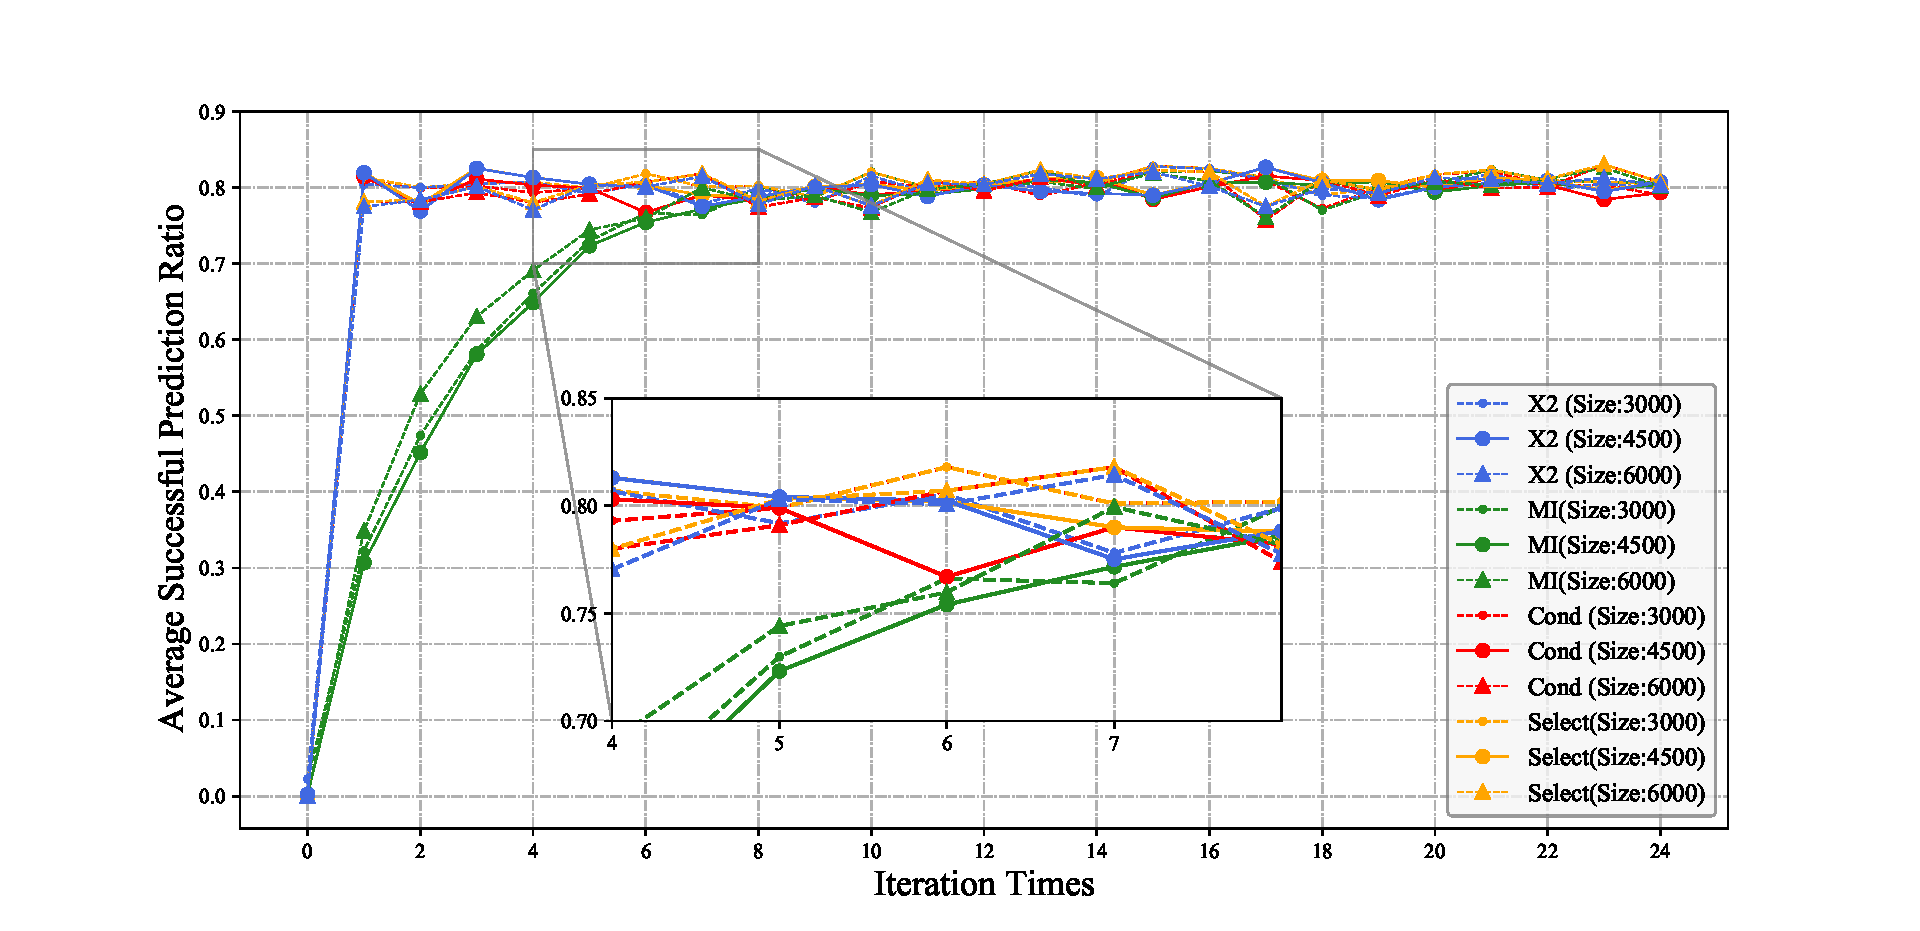
\includegraphics[height=6cm, width=11.5cm]{pre_accu} 
		\caption{The prediction performance of different correlation metrics} 
		\label{pic:prediction precision}
	\end{figure}

	\begin{figure}[t]
		\centering
		\vspace{-0.3cm}
		\begin{minipage}[c]{0.48\textwidth}
			\centering
			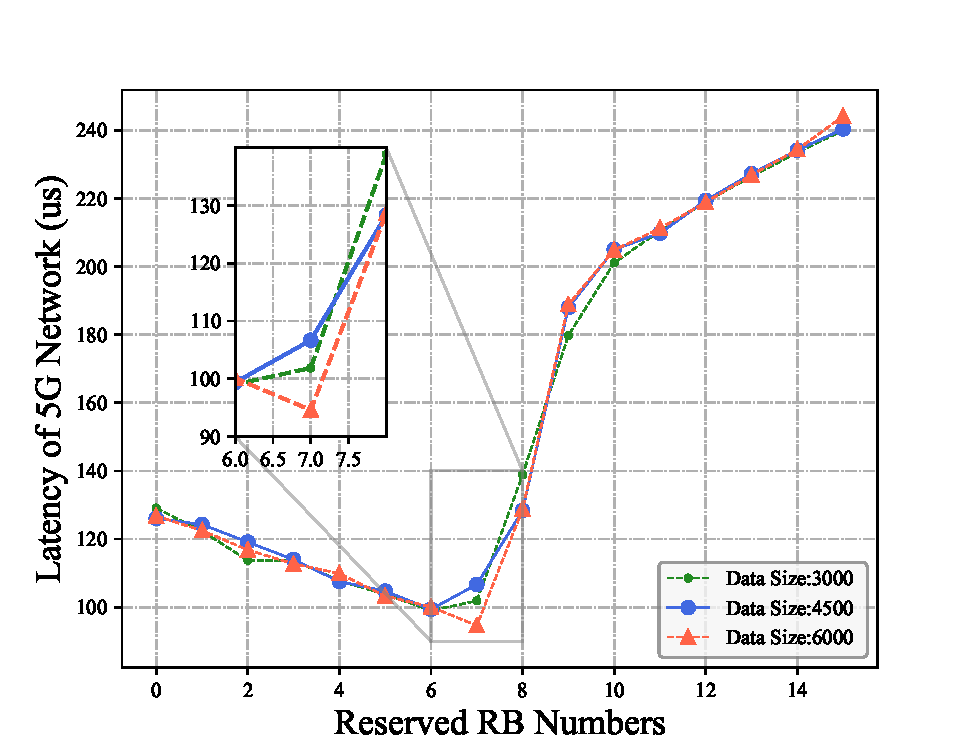
\includegraphics[width=8cm]{res_t5g}
		\end{minipage}
		\hspace{0.02\textwidth}
		\begin{minipage}[c]{0.48\textwidth}
			\centering
			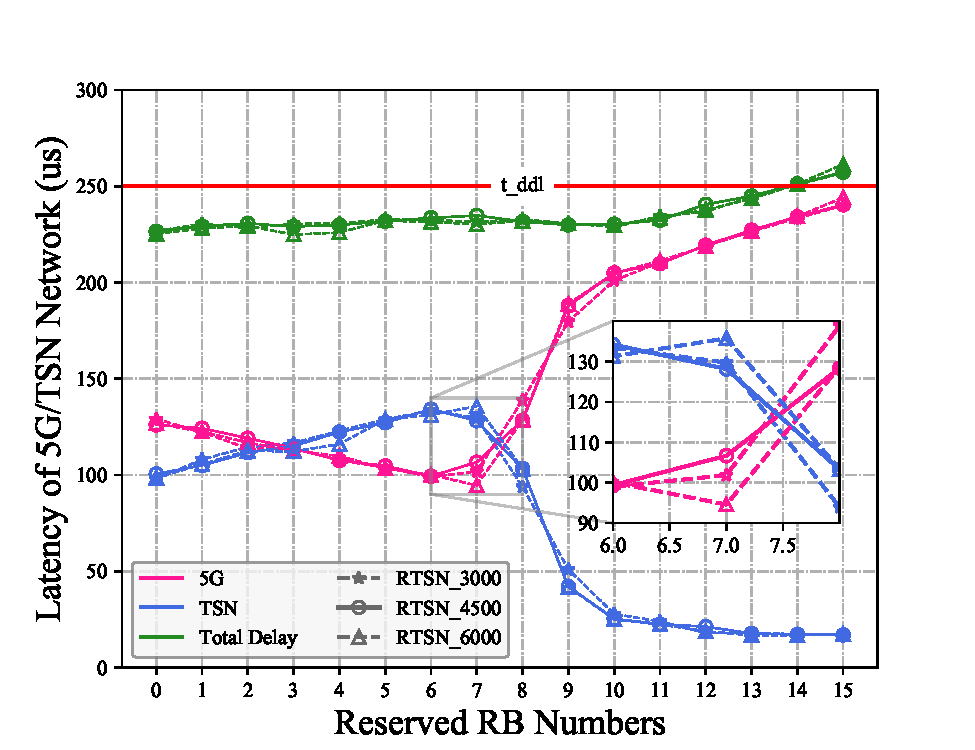
\includegraphics[width=8cm]{res_t5g_ttsn}
		\end{minipage}\\[3mm]
		\begin{minipage}[t]{0.48\textwidth}
			\centering 
			\caption{The varies of 5G delay with  $\left|\mathcal{R}_\mathrm{r}(t)\right|$}
			\label{fig:res-5g}
		\end{minipage}
		\hspace{0.02\textwidth}
		\begin{minipage}[t]{0.48\textwidth}
			\centering
			\caption{The varies of 5G and TSN delay with $\left|\mathcal{R}_\mathrm{r}(t)\right|$}
			\label{fig:res-5g/tsn}
		\end{minipage}
		\vspace{-0.3cm}
	\end{figure}


\begin{comment}
\begin{figure}[h]
	\centering
	\subfloat[test2]{
			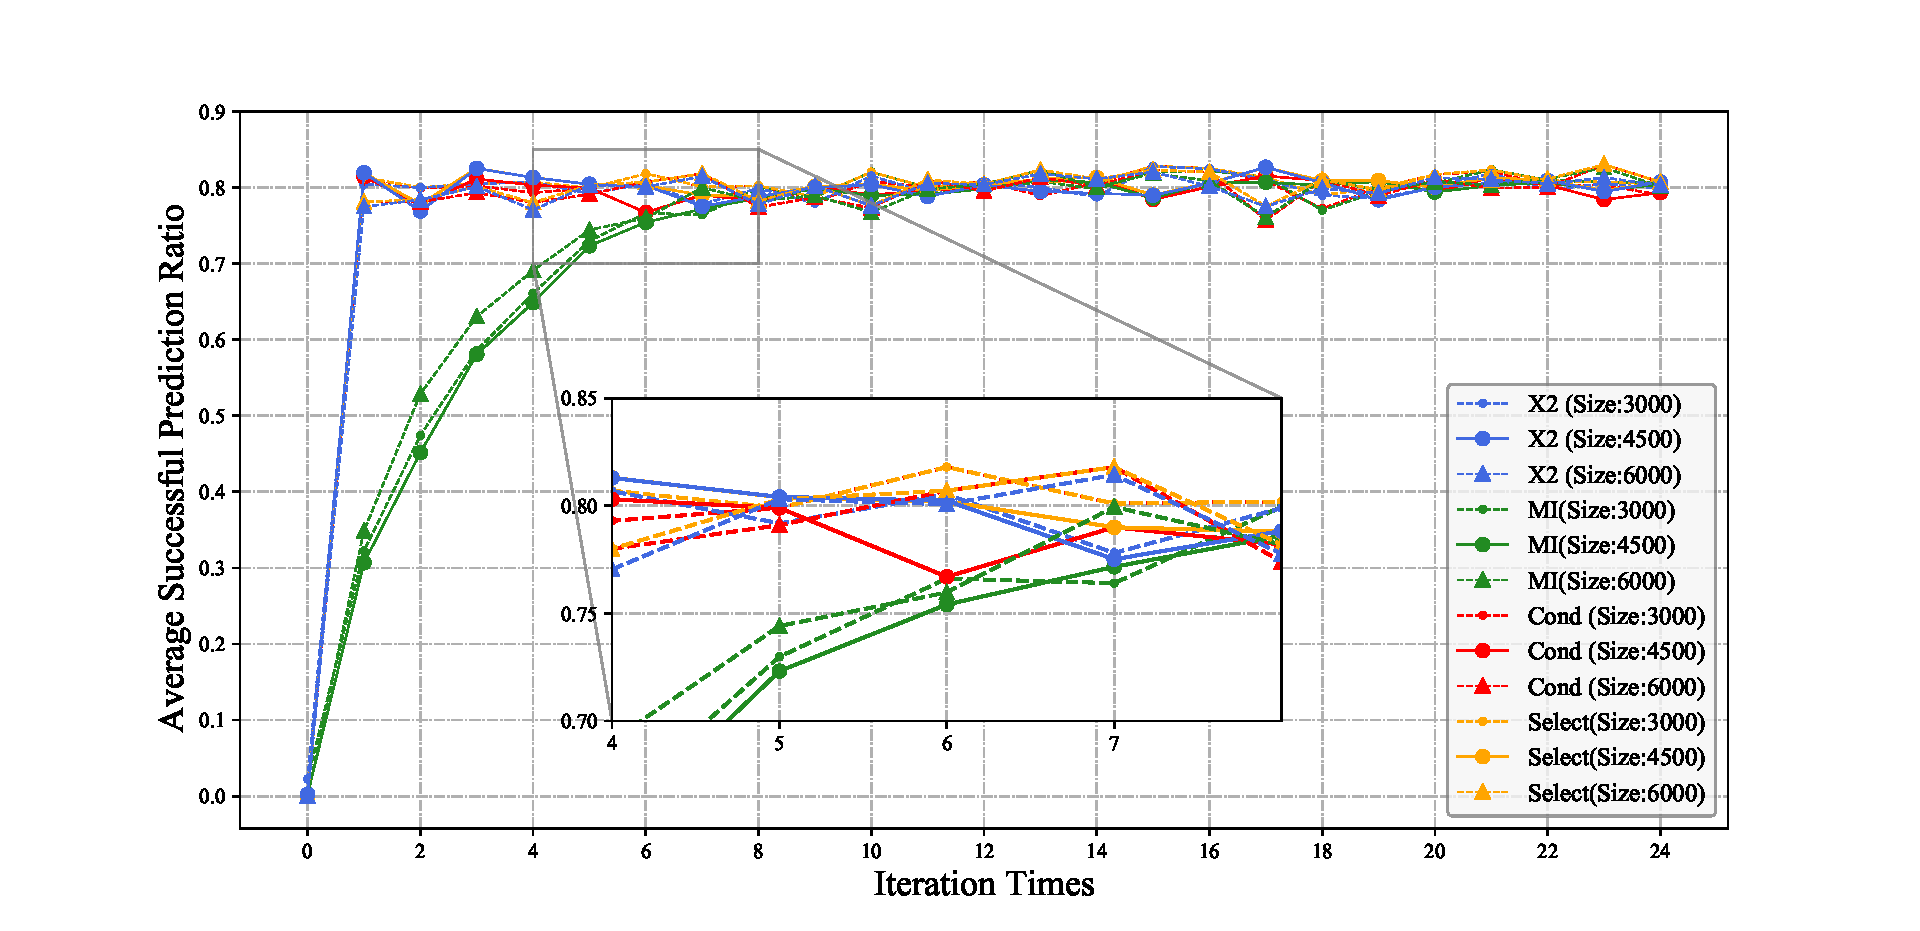
\includegraphics[width=0.5\textwidth]{pre_accu.pdf}
	}
	\subfloat[test2]{
		\begin{minipage}[b]{0.3\textwidth}
			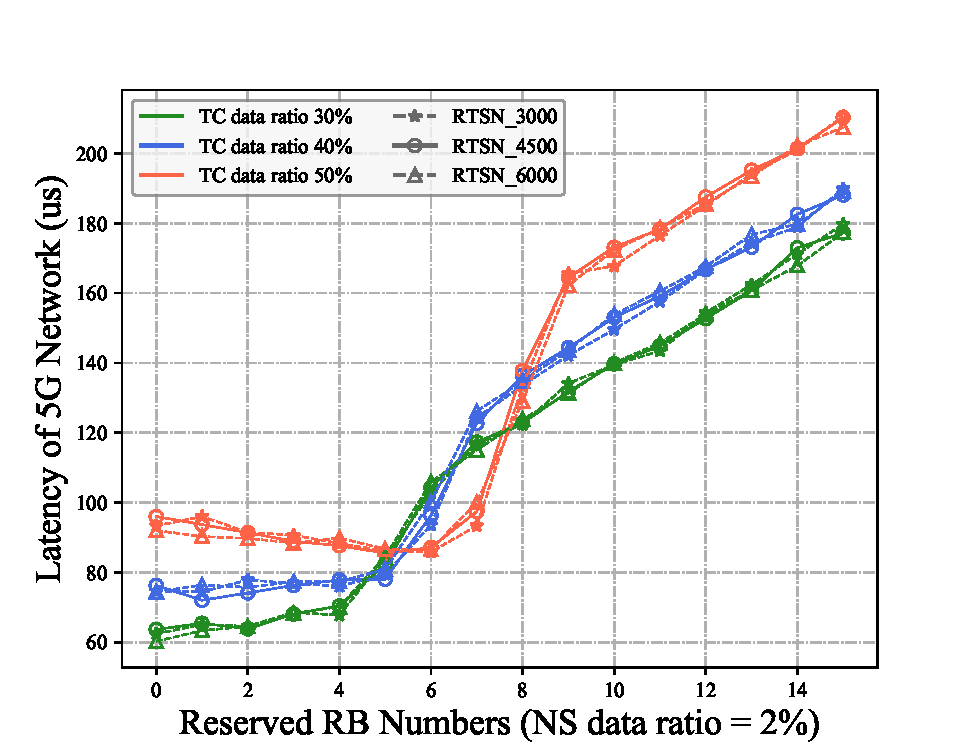
\includegraphics[align=c,width=1\textwidth]{t_5G_TC.pdf} \\
			\includegraphics[align=c,width=1\textwidth]{t_TSN_TC.pdf}
		\end{minipage}
		\hspace{-0.02\textwidth}
	}
	\subfloat[test2]{
		\begin{minipage}[b]{0.25\textwidth}
			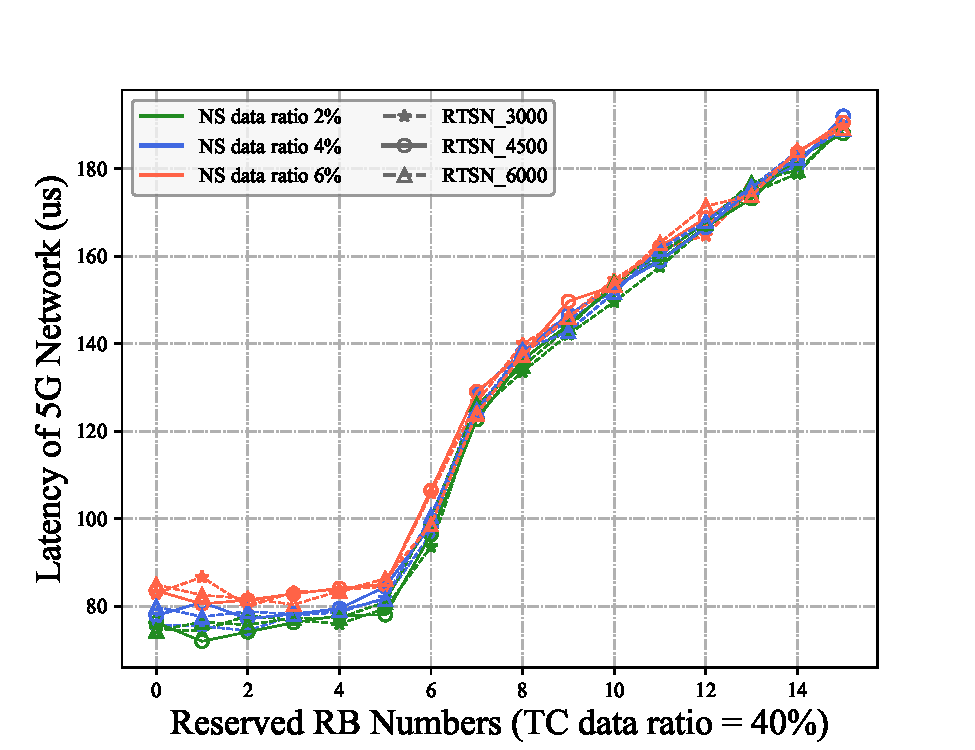
\includegraphics[align=c,width=1\textwidth]{t_5G_NS.pdf} 
		\end{minipage}
		\hspace{-0.02\textwidth}
	}

	\caption{subfigure test}
\end{figure}
\end{comment}

	
	\section{Numerical Results} 
	\label{result}
	\subsection{Sensor Prediction Simulation}~{}
	\par In this section, we evaluate the proposed HTSN architecture's performance based on data with a deterministic deadline, which generated by monitoring sensors deployed along the hot rolling line. Sensors for monitoring temperature, humidity, pressure are randomly distributed to sense the manufacturing process to provide robust control via closed-loop feedback. Sensors active periodically and generate TC data, which is the main type of data we care about. Event-triggered sensors such as camera and vibration sensors only active as long as there occur safety emergencies suddenly. They generate burst NS data, which has the highest priority and can preempt TC data.
	\par Here, data from different processes with its particular transmission deadline is transmitted in turns. What we need to do is to learn the correlation between sensors and despite the interference brought by sensors that have no relationship with the arrivals of steels. We consider the probability and proportion of field sensors as Table~\ref{tal:trigger paremeter}.
	\begin{table}[b]
		\footnotesize
		\caption{\textbf{Trigger of Sensors Setting}}
		\label{tal:trigger paremeter}
		\label{tab1}
		\tabcolsep 38pt %space between two columns.
		\begin{tabular*}{\textwidth}{cccc}
			\toprule
			\textbf{Proportion} & \textbf{NS data} & \textbf{TC data} & \textbf{BE data}\\\hline
			Proportion 1 & 6\% & 40\% & 54\% \\
			Proportion 2 & 4\% & 40\% & 56\% \\
			Proportion 3 & 2\% & 40\% & 58\% \\
			Proportion 4 & 2\% & 50\% & 48\% \\
			Proportion 5 & 2\% & 30\% & 68\% \\
			\bottomrule
		\end{tabular*}
	\end{table}
	
	\par  The performance of the predictive sensor selection algorithm (SSA) is evaluated in terms of prediction accuracy(successful prediction ratio). We compare the performance of three correlation metrics(X2: Chi-square test, MI: Mutual Information, Cond: Conditional Probability) and the sensor selection algorithm we proposed on three sizes(3000, 4500, 6000) of data. Figure~\ref{pic:prediction precision} shows how different correlation metrics diverse in the performance of prediction accuracy. It is obvious that the $\chi^{2}$ metric, as well as the conditional metric has the best performance while the iteration times are few. The prediction accuracy of Mutual Information is much lower and flat than the other two. But after several times of iteration, the difference between these three metrics' performance is inconspicuous, and the prediction accuracy of them all converges to 0.8. Since the SSA algorithm we proposed chooses the metric by threshold $\alpha$ and $\beta$, the performance of it is as good as the best metric. The high prediction accuracy guarantees the resource utilization of 5G and lays the foundation for the HTSN architecture.
	
	
	\subsection{HTSN Simulation}~{}
	\par Since the 5G network and TSN are coupling and interactive, the main influence factor of HTSN is the number of reserved RBs $\left|\mathcal{R}_\mathrm{r}(t)\right|$. Thus, we simulate the relationship between $\left|\mathcal{R}_\mathrm{r}(t)\right|$ and delay of 5G/TSN. Figure~\ref{fig:res-5g} shows that as $\left|\mathcal{R}_\mathrm{r}(t)\right|$ growing, the delay of the 5G network decrease firstly and then increases. The lowest point of the delay curve is the trade-off point we mentioned before, which is because the prediction accuracy cannot reach 100$\%$, thus assigning sensors in prior would cause the waste of radio resources. Here we set the total number of $Subslot$ to 15, and when $\left|\mathcal{R}_\mathrm{r}(t)\right|=7$, the performance of the pre-allocation mechanism is optimal. What's more, the reason why the delay of 5G network increases rapidly after the trade-off point is the limitation of radio resource, since the more $\left|\mathcal{R}_\mathrm{r}(t)\right|$ is reserved, the more resource is wasted accordingly, the fewer resources used for dynamic access and the lower reliability of transmission.
	
\begin{comment}
%显示t_5g-Rrt和t_5g-t_tsn
	\begin{figure}[t]
		\centering
		\vspace{-0.3cm}
		\begin{minipage}[c]{0.48\textwidth}
			\centering
			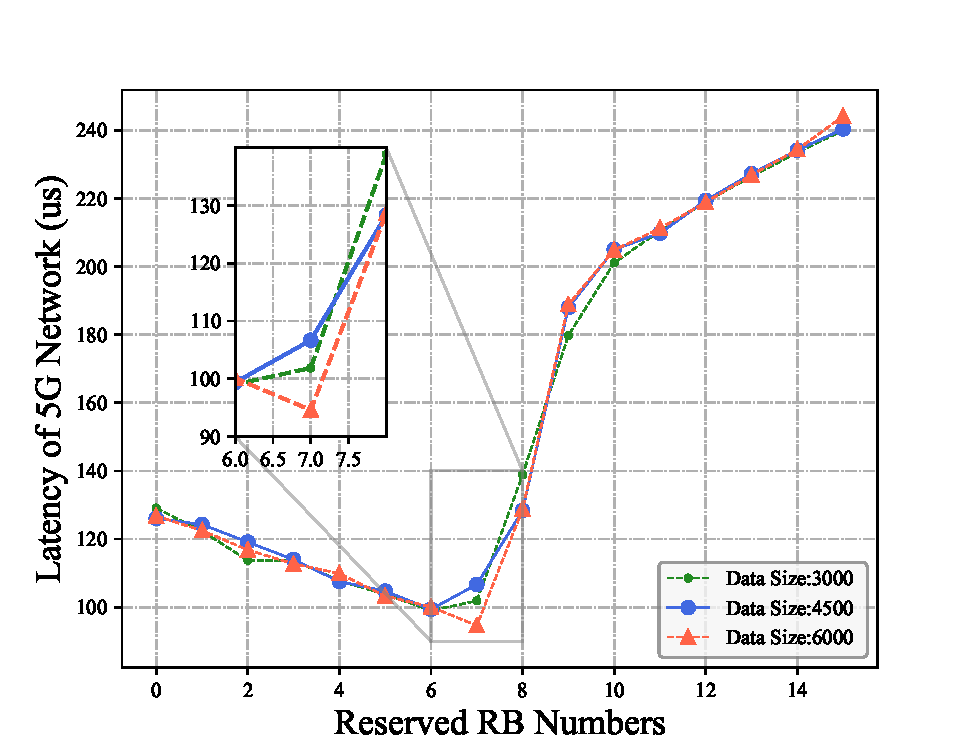
\includegraphics[width=8cm]{res_t5g}
		\end{minipage}
		\hspace{0.02\textwidth}
		\begin{minipage}[c]{0.48\textwidth}
			\centering
			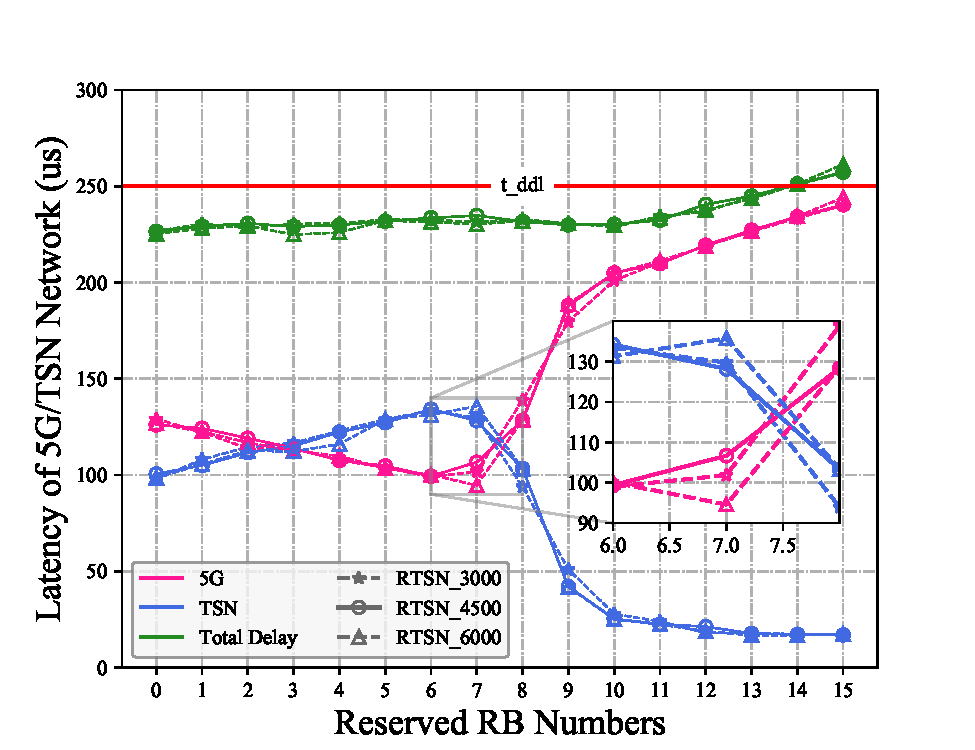
\includegraphics[width=8cm]{res_t5g_ttsn}
		\end{minipage}\\[3mm]
		\begin{minipage}[t]{0.48\textwidth}
			\centering 
			\caption{The varies of 5G delay with  $\left|\mathcal{R}_\mathrm{r}(t)\right|$}
			\label{fig:res-5g}
		\end{minipage}
		\hspace{0.02\textwidth}
		\begin{minipage}[t]{0.48\textwidth}
			\centering
			\caption{The varies of 5G and TSN delay with $\left|\mathcal{R}_\mathrm{r}(t)\right|$}
			\label{fig:res-5g/tsn}
		\end{minipage}
		\vspace{-0.3cm}
	\end{figure}



%显示t_5g-qt和t_5g-signal
	\begin{figure}[!t]
		\centering
		\begin{minipage}[c]{0.48\textwidth}
			\centering
			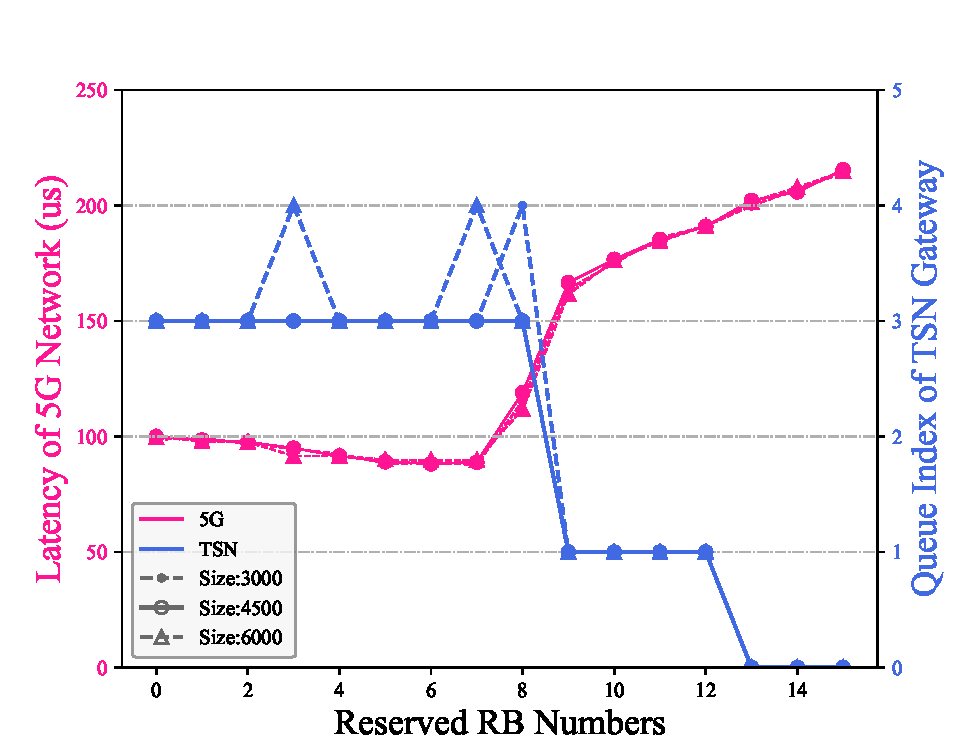
\includegraphics[width=8.25cm]{res_t5g_qt}
		\end{minipage}
		\hspace{0.02\textwidth}
		\begin{minipage}[c]{0.48\textwidth}
			\centering
			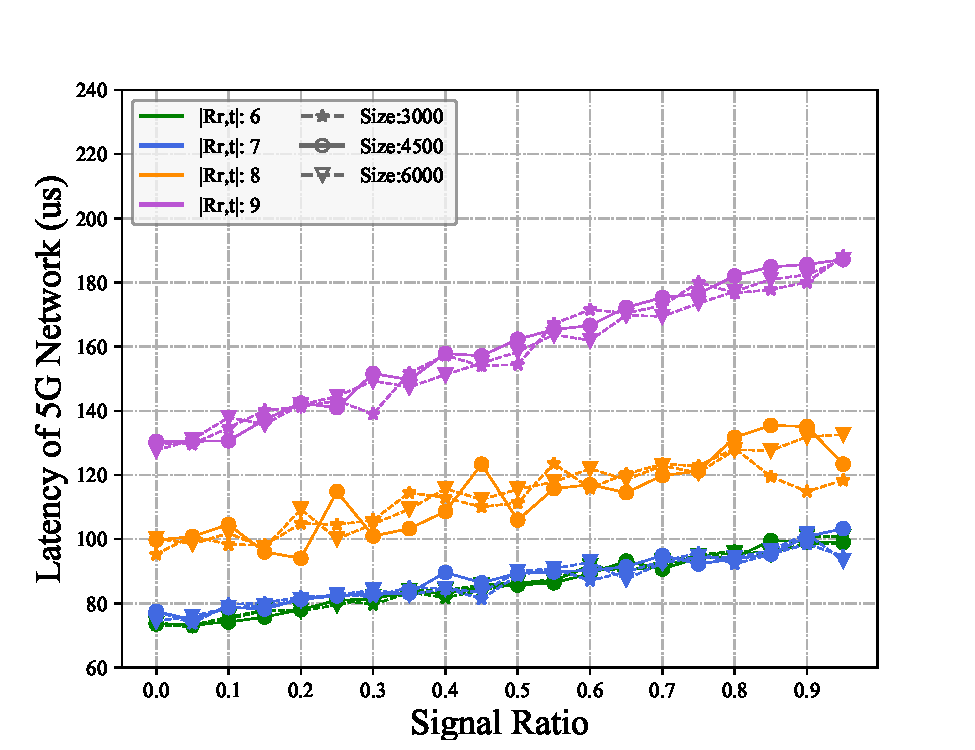
\includegraphics[width=8.25cm]{signal_t5g}
		\end{minipage}\\[3mm]
		\begin{minipage}[t]{0.48\textwidth}
			\centering
			\caption{The varies of Queue index and 5G delay with $\left|\mathcal{R}_\mathrm{r}(t)\right|$}
			\label{fig:q_5g}
		\end{minipage}
		\hspace{0.02\textwidth}
		\begin{minipage}[t]{0.48\textwidth}
			\centering
			\caption{The varies of 5G delay with signal ratio}
			\label{fig:signal-5g}
		\end{minipage}
	\end{figure}


%不用了的2×2排版
	\begin{figure}[t]
		%\begin{tabular}{cc}
		\begin{minipage}{0.5\linewidth}
			\centerline{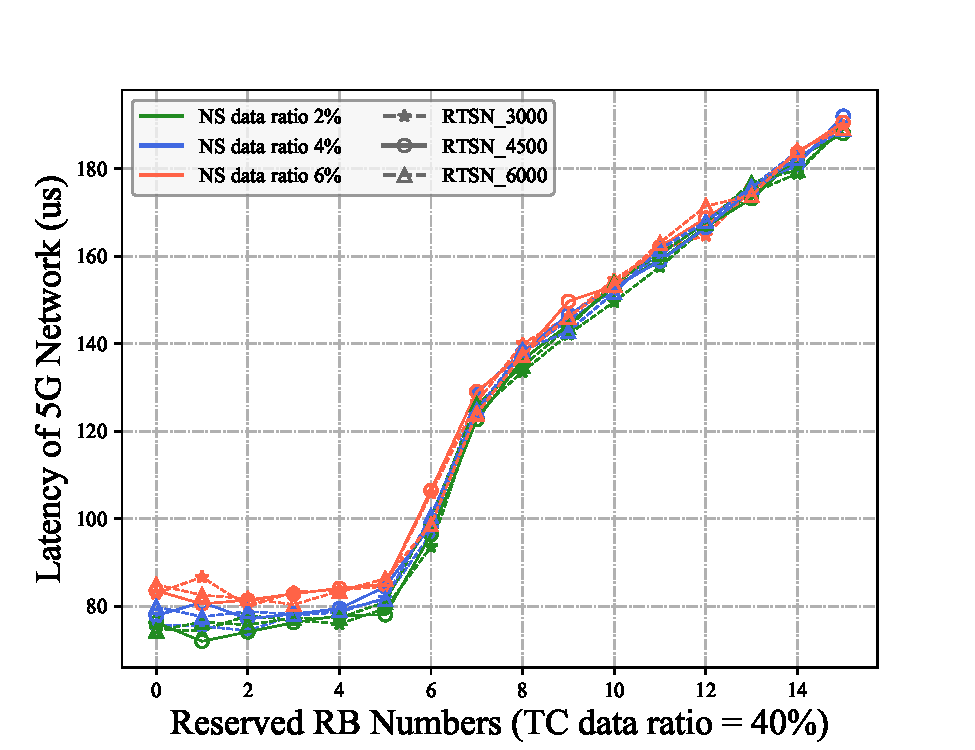
\includegraphics[width=8.0cm]{t_5G_NS.pdf}}
			\centerline{(a) 5G delay with TC data ratio = 40\%}
		\end{minipage}
		\hfill
		\begin{minipage}{0.5\linewidth}
			\centerline{\includegraphics[width=8.0cm]{t_TSN_NS.pdf}}
			\centerline{(b) TSN delay with TC data ratio = 40\%}
		\end{minipage}
		\vfill
		\begin{minipage}{0.5\linewidth}
			\centerline{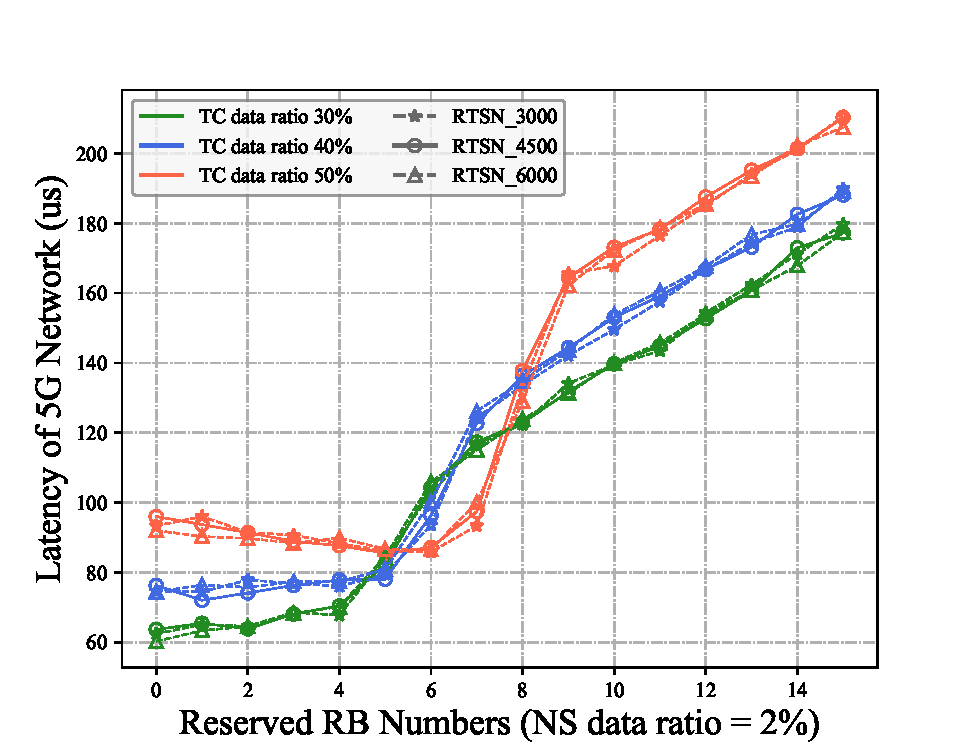
\includegraphics[width=8.0cm]{t_5G_TC.pdf}}
			\centerline{(c) 5G delay with NS data ratio = 2\%}
		\end{minipage}
		\hfill
		\begin{minipage}{0.5\linewidth}
			\centerline{\includegraphics[width=8.0cm]{t_TSN_TC.pdf}}	
			\centerline{(d) TSN delay with NS data ratio = 2\%}	
		\end{minipage}
		%\end{tabular}
		\caption{The varies of TC data's delay with  $\left|\mathcal{R}_\mathrm{r}(t)\right|$}
		\label{fig:res}
	\end{figure}
	
	\end{comment}



	\begin{figure}[t]
		\centering
		\subfloat{
			\begin{minipage}[b]{0.33\textwidth}
				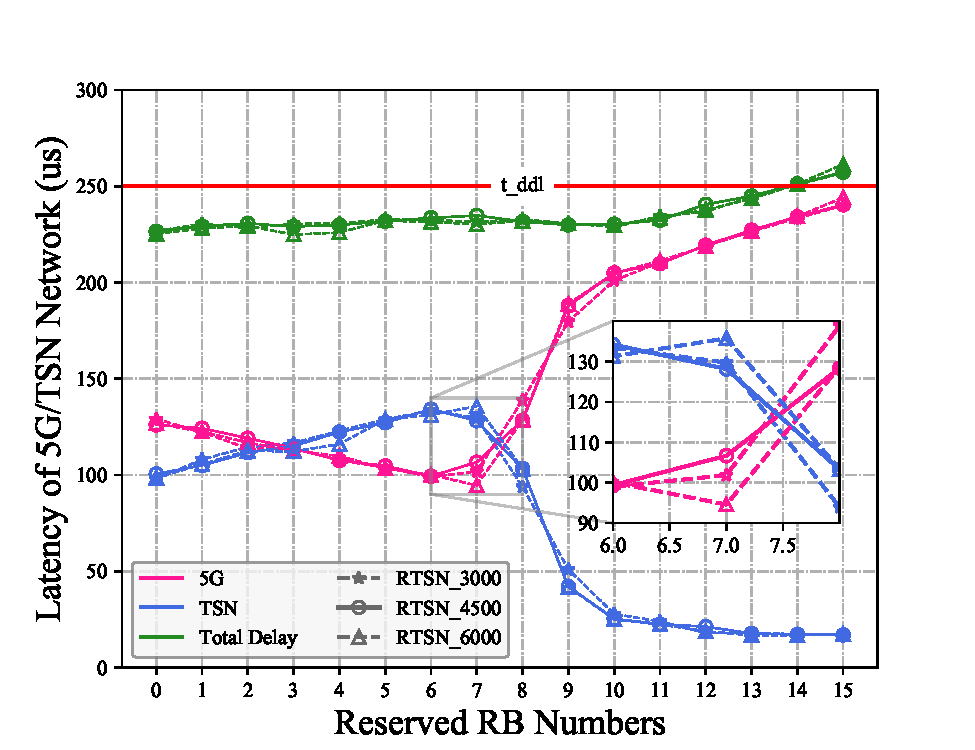
\includegraphics[width=1\textwidth]{res_t5g_ttsn.pdf} \\
				\vspace{-0.65cm}
				\caption{aa}
				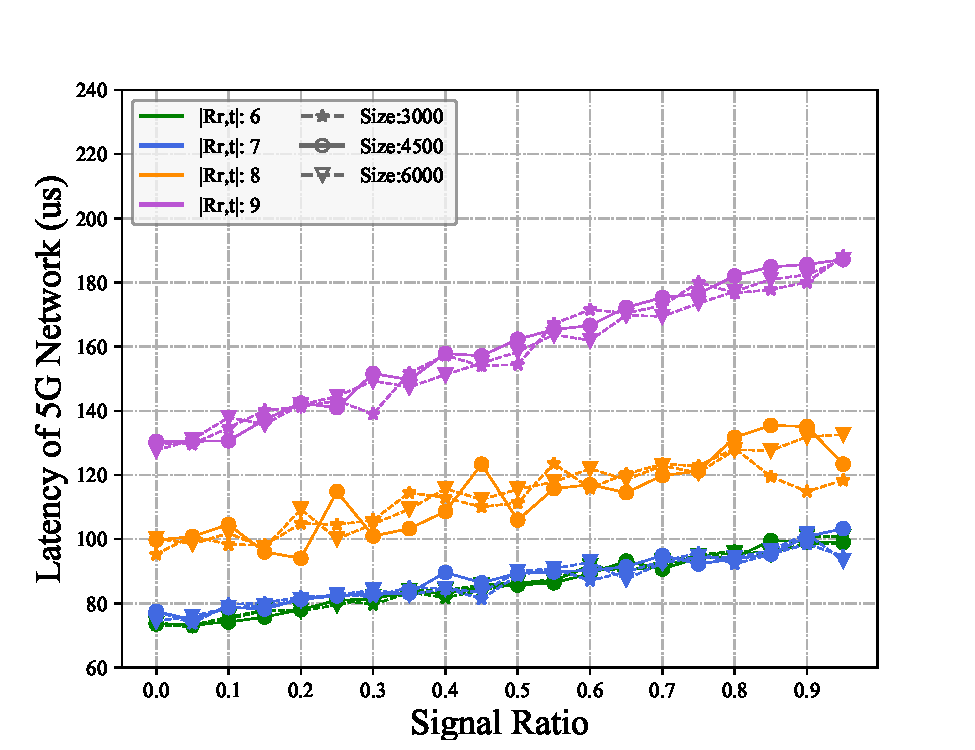
\includegraphics[width=1\textwidth]{signal_t5g.pdf} 
				\vspace{-0.65cm}
				\caption{bb}
			\end{minipage}
			%\hspace{-0.02\textwidth} %调整列间距
		}
	%将补充仿真跟pre_accu放到一起
		\subfloat[test2]{
			\begin{minipage}[b]{0.33\textwidth}
				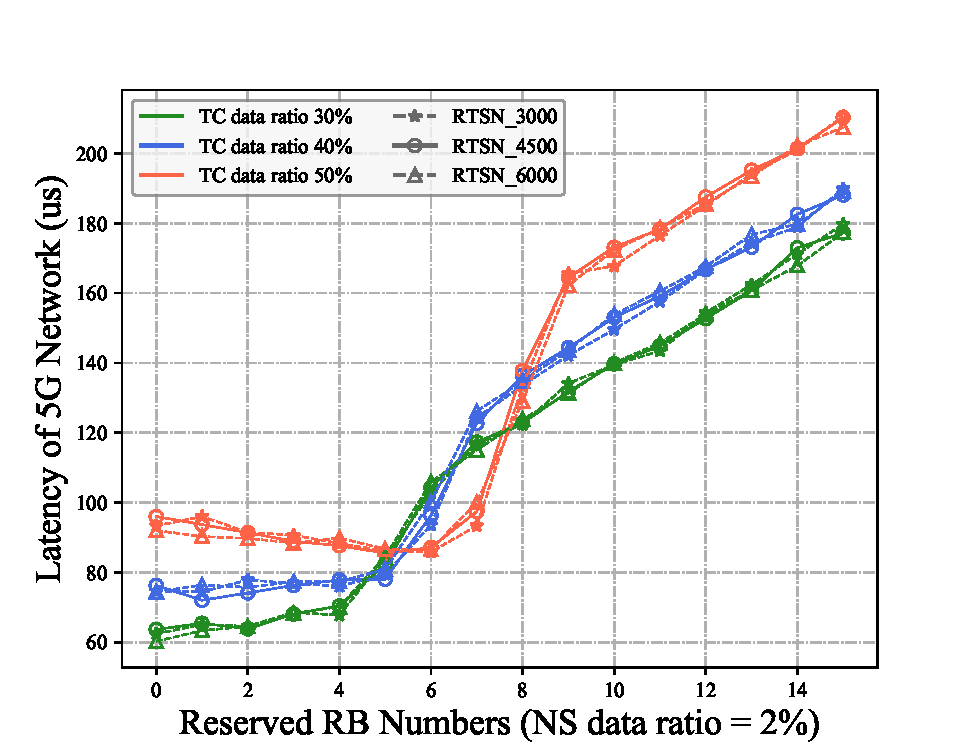
\includegraphics[width=1\textwidth]{t_5G_TC.pdf} \\
				\includegraphics[width=1\textwidth]{t_TSN_TC.pdf}
			\end{minipage}
		\hspace{-0.02\textwidth}
		}
		\subfloat[test2]{
			\begin{minipage}[b]{0.33\textwidth}
				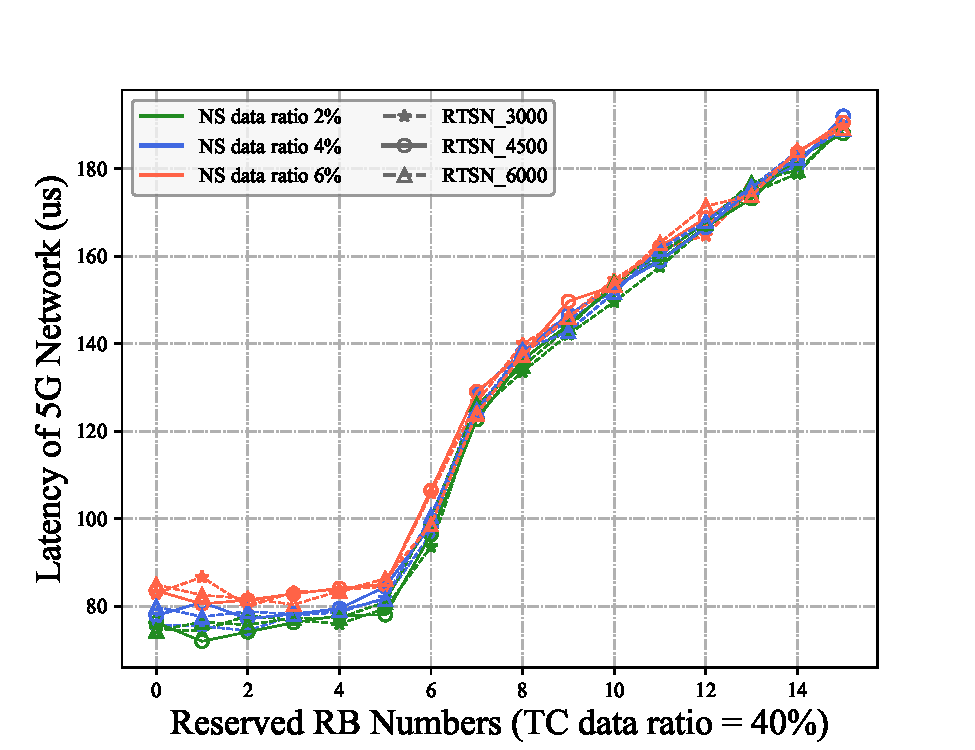
\includegraphics[width=1\textwidth]{t_5G_NS.pdf} \\
				\includegraphics[width=1\textwidth]{t_TSN_NS.pdf}
			\end{minipage}
		\hspace{-0.02\textwidth}
		}
		
		\caption{subfigure test}
	\end{figure}




\begin{comment}
	\begin{figure*}[htbp] 
		\begin{center} 
			\footnotesize 
			\tabcolsep -5pt
			\begin{tabular}{cccc} 
				\includegraphics[scale=0.3]{t_TSN_TC.pdf} & 
				\includegraphics[scale=0.3]{t_TSN_TC.pdf} & 
				\includegraphics[scale=0.3]{t_TSN_TC.pdf} & 
				\includegraphics[scale=0.3]{t_TSN_TC.pdf}\\ 
				%(a) dCOEA &(b) PPS-RM &(c) DEE-DMOEA\\ 
				a & b & c & d\\ 
				\includegraphics[scale=0.3]{t_TSN_TC.pdf}~~&~~ 
				\includegraphics[scale=0.3]{t_TSN_TC.pdf}~~&~~ 
				\includegraphics[scale=0.3]{t_TSN_TC.pdf}~~&~~ 
				\includegraphics[scale=0.3]{t_TSN_TC.pdf}\\ 
				%(a) dCOEA &(b) PPS-RM &(c) DEE-DMOEA\\ 
				a & b & c & d\\ 
			\end{tabular} 
		\end{center} 
		\caption{Solution sets founded by three algorithms at eight different time steps on F3.} 
		\label{Fig:F3} 
	\end{figure*}
\end{comment}

	
	\par Based on the dynamic injection of the TSN queue, the indeterminacy of transmission caused by the 5G network can be made up by the TSN to meet the strict transmission requirements of intelligent manufacturing. Figure~\ref{fig:res-5g/tsn} shows the interaction of 5G and TSN as $\left|\mathcal{R}_\mathrm{r}(t)\right|$ growing. It can be seen that the delay of 5G and TSN has a near-ideal negative correlation via adjusting the TSN queue priority self-adaptively. Given the deadline = 250$\mu$s, the TSN tries to save as many resources as it can under the premise of not violating the deadline of the total delay under HTSN. Obviously, the data injection mechanism we proposed makes up for the shortcoming of the 5G network perfectly and improves the determinacy since it nearly not violates the deadline.
	
	\par To further analyze the relationship between TSN queue and 5G delay, we give Figure~\ref{fig:q_5g}, from which we can see that the IPV number of data and the 5G network delay also have a similar negative correlation. Since the IPV number of data is directly proportional to its TSN delay, the general trend of the queue priority curve and TSN delay curve is analogous. However, there are some step-changes of the IPV number as it is an integer. It can also be concluded that although we arrange a IPV number between 0 and 8, we can't assign 5G data to the queue correspongding to IPV 8 since the scheduling capability of the 5G network is not enough to realize low latency high-reliability transmission by itself.
	
	\begin{figure}[t]
		\vspace{-0.2cm}
		\centering 
		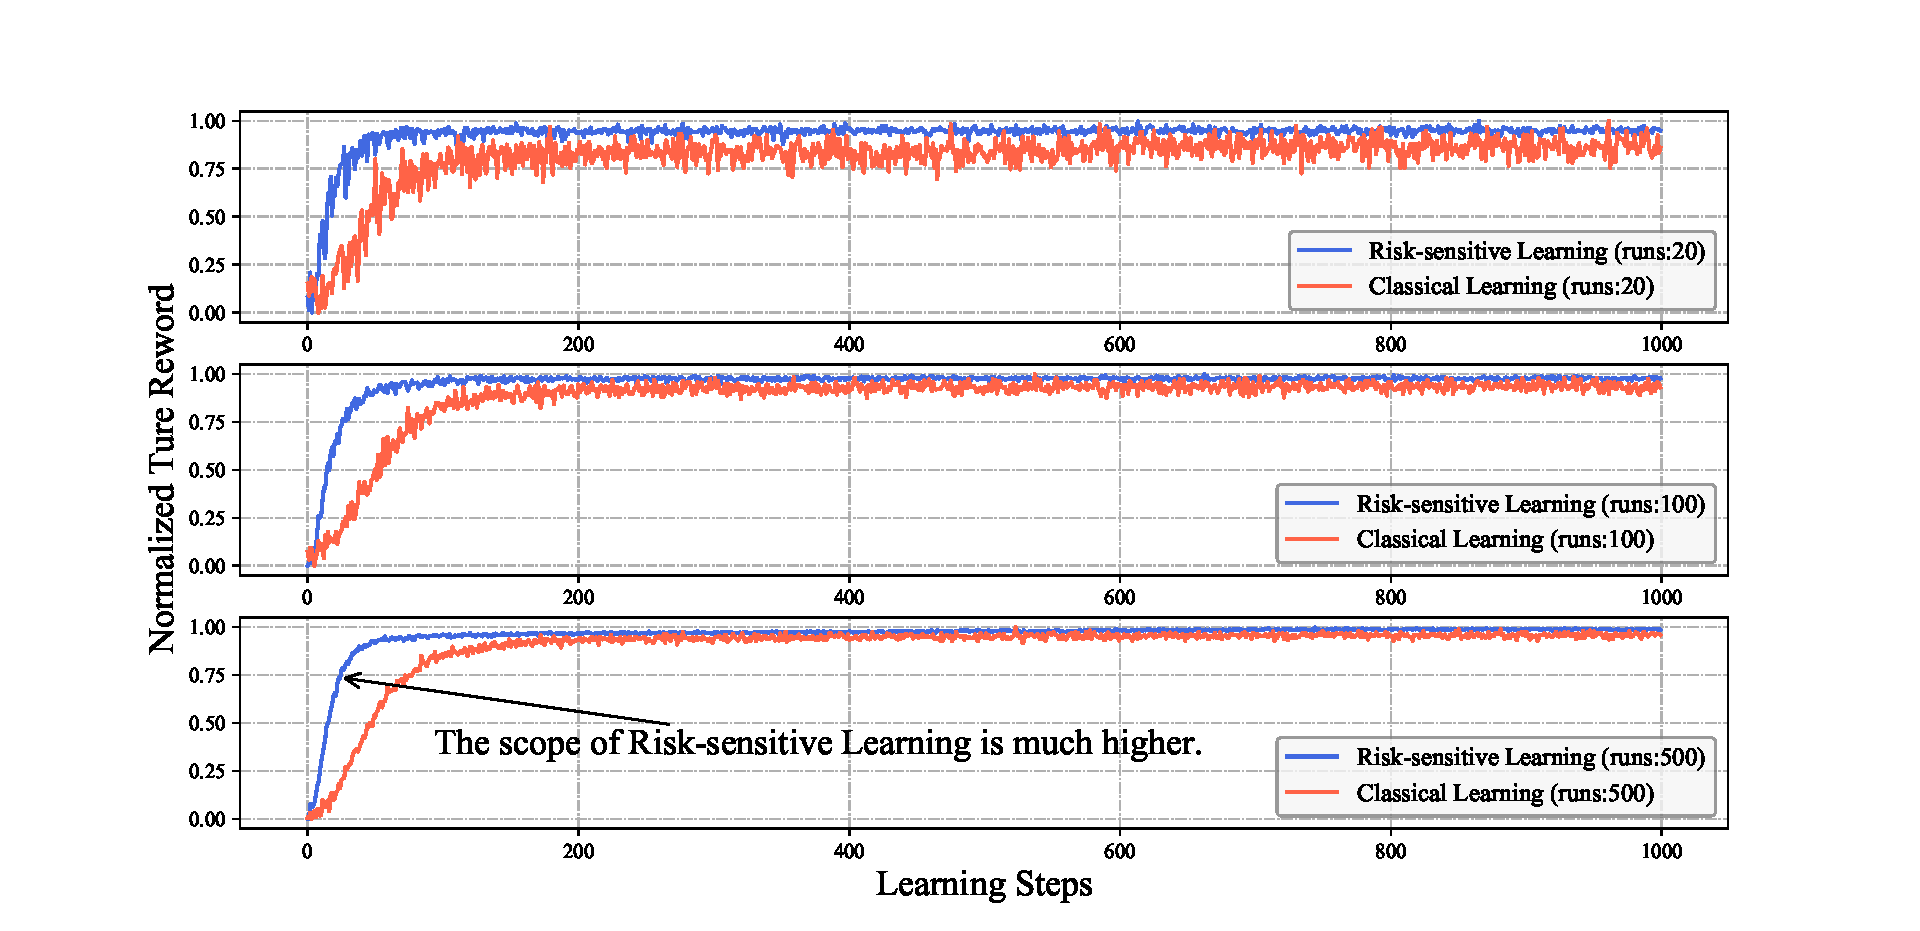
\includegraphics[height=6.3cm, width=13cm]{RSL} 
		\caption{The normalized reward of risk-sensitive reinforcement learning with different run times} 
		\label{fig:risk reward}
	\end{figure}
	
	\begin{figure}[t]
		\vspace{-0.2cm}
		\centering 
		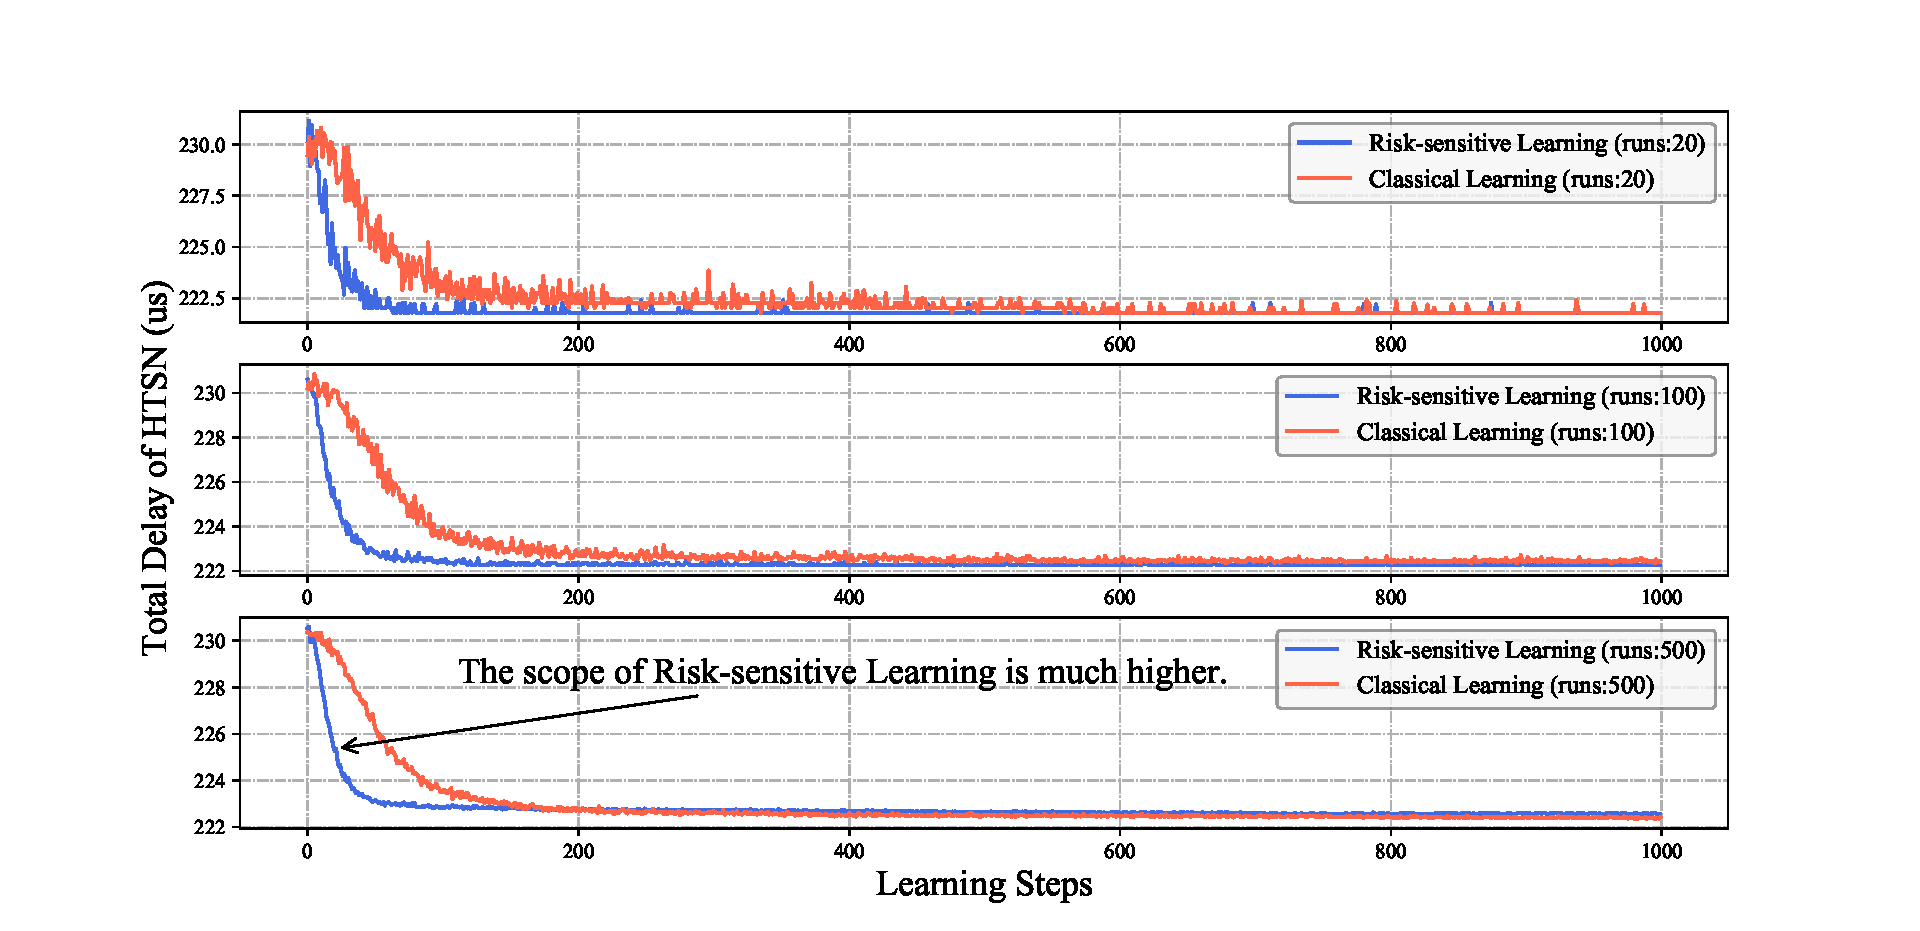
\includegraphics[height=6.3cm, width=13cm]{risk_delay} 
		\caption{The total delay of HTSN with different learning run times} 
		\label{fig:risk_delay}
	\end{figure}
	
	\par Except for $\left|\mathcal{R}_\mathrm{r}(t)\right|$, the ratio of signaling transmission is also a critical factor that influences the SPS within the 5G network and the total delay of HTSN. Here, we formulate the extra delay caused by signaling as a signal ratio and plot the relationship between it and 5G delay. As Figure~\ref{fig:signal-5g} shows, we select $\left|\mathcal{R}_\mathrm{r}(t)\right|$ from 6 to 9 according to Figure~\ref{fig:res-5g} to find the influence among signal ratio, $\left|\mathcal{R}_\mathrm{r}(t)\right|$ and delay of 5G. It can be seen that no matter $\left|\mathcal{R}_\mathrm{r}(t)\right|$ is larger, equal, or less than the trade-off point, the delay of 5G network increases with the increase of signal ratio. This is because $\left|\mathcal{R}_\mathrm{r}(t)\right|$ has nothing to do with the number of TC data; there always exists TC data to be dynamically scheduled due to the inaccuracy of prediction, so the increase of signal ratio will lead to the increase of the 5G network's delay.
	
	
	\subsection{Risk-sensitive Learning Simulation}~{}
	\par To deal with the tail of 5G delay, we use a risk-sensitive utility function to optimize expectations and high order quantities of accumulative integral delay of HTSN. The proposed HTSN architecture is evaluated as an integral in Figure~\ref{fig:risk reward}, which delineates the improvement brought by the risk-sensitive utility. We repeat GMAB learning for three sizes (20,100,500) of independent runs, and each run we measure its performance with experience over 1000 time steps. With the increase of repetitions, the risk-sensitive learning curve is more stable, and the learning reward is getting closer to the normalized true reward. It means that the learning rate of risk-sensitive learning is faster than classical learning. Besides, with the increase of iteration times, the convergence rate of risk-sensitive learning is faster.
	
	\par As for the performance of the total delay shown in Figure~\ref{fig:risk_delay}, the curve of Figure~\ref{fig:risk reward} and Figure~\ref{fig:risk_delay} are analogous with the same parameter settings. It can be seen that the curve of risk-sensitive learning is steeper than the classical one, which means that the high order quantities are optimized while learning, and the delay distribution of HTSN is more centralized with a shorter tail. It proves the risk-sensitive reinforcement learning strategy we proposed works and develops the transmission reliability.
	
	
	\section{Conclusion} 
	\label{con}
	\par In this paper, we proposed HTSN, a heterogeneous architecture that co-designs 5G and TSN to provide deterministic transmission from the industrial field to the remote data center. Within the 5G network, a preemption considered multi-priority wireless scheduling mechanism was proposed to satisfy the diverse QoS requirements of field data by exploring the trigger correlation between uplink sensors in industrial process automation. To offset the indeterminacy caused by the 5G network, an adaptive data injection mechanism of the TSN gateway queue was developed here to reduce the total delay under HTSN. Then we formulated a risk-sensitive utility function, which considers the high order quantity of the total dealy into account. Finally, a risk-sensitive reinforcement learning based on GMAB is executed and thus the determinacy of HTSN is improved.
	
	
	%\theorem[name]{It is a test theorem.}
	
	
	
	%%%%%%%%%%%%%%%%%%%%%%%%%%%%%%%%%%%%%%%%%%%%%%%%%%%%%%%
	%%% Acknowledgements. 
	%%%%%%%%%%%%%%%%%%%%%%%%%%%%%%%%%%%%%%%%%%%%%%%%%%%%%%%
	%\Acknowledgements{This work was supported by National Natural Science Foundation of China (Grant Nos. 00000000 and 11111111).}
	
	
	%%%%%%%%%%%%%%%%%%%%%%%%%%%%%%%%%%%%%%%%%%%%%%%%%%%%%%%
	%%% Supplements. 
	%%%%%%%%%%%%%%%%%%%%%%%%%%%%%%%%%%%%%%%%%%%%%%%%%%%%%%%
	%\Supplements{Appendix A.}
	
	%%%%%%%%%%%%%%%%%%%%%%%%%%%%%%%%%%%%%%%%%%%%%%%%%%%%%%%
	%%% Reference section.
	%%% citation in the content using "some words~\cite{1,2}".
	%%% ~ is needed to make the reference number is on the same line with the word before it.
	%%%%%%%%%%%%%%%%%%%%%%%%%%%%%%%%%%%%%%%%%%%%%%%%%%%%%%%
	
	\begin{comment}
	\bibliographystyle{unsrt}
	\begin{thebibliography}{99}
	
	\bibitem{3} Li M, Guan X, Hua C, et al. Predictive pre-allocation for low-latency uplink access in industrial wireless networks. IEEE INFOCOM-IEEE Conference on Computer Communications, Honolulu, USA, 2018. 306-314
	
	\bibitem{25} Li M, Chen C, Hua C, et al. A Learning-Based Pre-Allocation Scheme for Low-Latency Access in Industrial Wireless Networks. IEEE Trans Wirel Commun, 2019, 19(1): 650-664.
	
	\bibitem{26} János F, Balázs V, György M, et al. 5G-TSN integration meets networking requirements for industrial automation. Ericsson Technology Review, 2019.
	
	\bibitem{30} Fu S, Wu J, Wen H, et al. Software defined wireline-wireless cross-networks: Framework, challenges, and prospects. IEEE Commun Mag, 2018, 56(8): 145-151.
	
	\bibitem{31} Ke C H, Chen Y S, Yu Y S. Improving video transmission in software defined wired and wireless networks using multi-path transmission. J Commun Netw, 2017, 19(6): 587-595.
	
	\bibitem{32} Cai L, Shen X S, Mark J W, et al. QoS support in wireless/wired networks using the TCP-friendly AIMD protocol. IEEE Trans Wirel Commun, 2006, 5(2): 469-480.
	
	\bibitem{33} Underberg L, Kays R, Dietrich S, et al. Towards hybrid wired-wireless networks in industrial applications. IEEE Industrial Cyber-Physical Systems, Saint Petersburg, Russia, 2018: 768-773.
	
	\bibitem{35} Sachs J, Wallstedt K, Alriksson F, et al. Boosting smart manufacturing with 5G wireless connectivity. Ericsson Technology Review, 2019.
	
	\bibitem{5} Föllmer H, Schied A. Stochastic finance: an introduction in discrete time. Walter de Gruyter, 2011.
	
	\bibitem{6} Batewela S, Liu C F, Bennis M, et al. Risk-Sensitive Task Fetching and Offloading for Vehicular Edge Computing. IEEE Commun Lett, 2019, 24(3): 617-621.
	
	\bibitem{7} Bennis M, Debbah M, Poor H V. Ultrareliable and low-latency wireless communication: Tail, risk, and scale. Proc IEEE, 2018, 106(10): 1834-1853.
	
	\bibitem{8} Yang G, Xiao M, Poor H V. Low-latency millimeter-wave communications: data dispersion or network densification?. IEEE Trans Commun, 2018, 66(8): 3526-3539.
	
	\bibitem{9} Vu T K, Liu C F, Bennis M, et al. Path selection and rate allocation in self-backhauled mmWave networks. IEEE Wireless Communications and Networking Conference, Barcelona, Spain, 2018. 1-6.
	
	\bibitem{10} Vu T K, Liu C F, Bennis M, et al. Ultra-reliable and low latency communication in mmWave-enabled massive MIMO networks. IEEE Commun Lett, 2017, 21(9): 2041-2044.
	
	\bibitem{11} Assaad M, Ahmad A, Tembine H. Risk sensitive resource control approach for delay limited data in wireless networks. IEEE Global Telecommunications Conference-GLOBECOM,  Houston, Texas, USA, 2011. 1-5.
	
	\bibitem{12} Alsenwi M, Tran N H, Bennis M, et al. eMBB-URLLC resource slicing: A risk-sensitive approach. IEEE Commun Lett, 2019, 23(4): 740-743.
	
	\bibitem{13} Holfeld B, Wieruch D, Wirth T, et al. Wireless communication for factory automation: An opportunity for LTE and 5G systems. IEEE Commun Mag, 2016, 54(6): 36-43.
	
	\bibitem{14} 3GPP. Evolved Universal Terrestrial Radio Access (E-UTRA) and Evolved Universal Terrestrial Radio Access Network (E-UTRAN). 3gpp Ts, 2010.
	
	\bibitem{15} Schulz P, Matthe M, Klessig H, et al. Latency critical IoT applications in 5G: Perspective on the design of radio interface and network architecture.IEEE Commun Mag, 2017, 55(2): 70-78.
	
	\bibitem{16} Seo J B, Leung V C M. Performance modeling and stability of semi-persistent scheduling with initial random access in LTE. IEEE Trans Wirel Commun, 2012, 11(12): 4446-4456.
	
	\bibitem{17} Afrin N, Brown J, Khan J Y. Design of a buffer and channel adaptive LTE semi-persistent scheduler for M2M communications. IEEE International Conference on Communications, London, UK, 2015. 5821-5826.
	
	\bibitem{18} Soleymani D M, Puschmann A, Roth-Mandutz E, et al. A hierarchical radio resource management scheme for next generation cellular networks, IEEE Wireless Communications and Networking Conference Workshops, Doha, Qatar, 2016. 416-420.
	
	\bibitem{21} Raza M, Le-minh H, Aslam N, et al. A novel MAC proposal for critical and emergency communications in Industrial Wireless Sensor Networks. Comput Electr Eng, 2018, 72: 976-989.
	
	\bibitem{19} Farag H, Sisinni E, Gidlund M, et al. Priority-aware wireless fieldbus protocol for mixed-criticality industrial wireless sensor networks. IEEE Sens J, 2018, 19(7): 2767-2780.
	
	\bibitem{20} Gaj P, Jasperneite J, Felser M. Computer communication within industrial distributed environment—A survey. IEEE Trans Ind Inform, 2012, 9(1): 182-189.
	
	\bibitem{22} Zand P, Chatterjea S, Das K, et al. Wireless industrial monitoring and control networks: The journey so far and the road ahead. J Sens Actuator Netw, 2012, 1(2): 123-152.
	
	\bibitem{23} Lin F, Dai W, Li W, et al. A Framework of Priority-Aware Packet Transmission Scheduling in Cluster-Based Industrial Wireless Sensor Networks. IEEE Trans Ind Inform, 2019, 16(8): 5596-5606.
	
	\bibitem{24} Thu-Hang N T, Trinh N C, Ban N T, et al. Delay and reliability analysis of p-persistent carrier sense multiple access for multi-event industrial wireless sensor networks. IEEE Sens J, 2020.
	
	\bibitem{1} Lien S Y, Chen K C. Massive access management for QoS guarantees in 3GPP machine-to-machine communications. IEEE Commun Lett, 2011, 15(3): 311-313.
	
	\bibitem{2} Shafiq M Z, Liu A X, et al. Large-scale measurement and characterization of cellular machine-to-machine data. IEEE-ACM Trans Netw, 2013, 21(6): 1960-1973.
	
	\bibitem{4} Sanasam R, Murthy H, Gonsalves T. Feature selection for text classification based on gini coefficient of inequality. Feature Selection in data Mining, Hyderabad, India, 2010. 76-85.
	
	\bibitem{27} Arora P, Szepesvári C, Zheng R. Sequential learning for optimal monitoring of multi-channel wireless networks. IEEE Infocom, Shanghai, China, 2011.
	
	\bibitem{28} Xu Q, Zheng R. When data acquisition meets data analytics: A distributed active learning framework for optimal budgeted mobile crowdsensing, IEEE INFOCOM-IEEE Conference on Computer Communications, Atlanta, USA, 2017. 1-9.
	
	\bibitem{29} Sutton R S, Barto A G. Reinforcement learning: An introduction. MIT press, 2018.
	
	
	
	
	
	\end{thebibliography}
	\end{comment}
	%%%%%%%%%%%%%%%%%%%%%%%%%%%%%%%%%%%%%%%%%%%%%%%%%%%%%%%
	%%% Appendix sections.
	%%%%%%%%%%%%%%%%%%%%%%%%%%%%%%%%%%%%%%%%%%%%%%%%%%%%%%%
	%\begin{appendix}
	%\section{Name}
	
	%\end{appendix}
	\bibliography{reference}
\end{document}


%%%%%%%%%%%%%%%%%%%%%%%%%%%%%%%%%%%%%%%%%%%%%%%%%%%%%%%
%%% Some latex examples for this template
%%%%%%%%%%%%%%%%%%%%%%%%%%%%%%%%%%%%%%%%%%%%%%%%%%%%%%%

%%% sections. 
\section{Section title}
\subsection{Subsection title}
\subsubsection{Subsubsection title}


%%% list.
\begin{itemize}
	\item Aaa aaa.
	\item Bbb bbb.
	\item Ccc ccc.
\end{itemize}

%%% list-with-other-label. 
\begin{itemize}
	\itemindent 2.8em
	\item[(1)] Aaa aaa.
	\item[(2)] Bbb bbb.
	\item[(3)] Ccc ccc.
\end{itemize}

%%% Theorem-like section. 
%%% [name] can be ommited. [name]
\assumption[name]{Content.}
\corollary[name]{Content.}
\definition[name]{Content.}
\example[name]{Content.}
\lemma[name]{Content.}
\problem[name]{Content.}
\proposition[name]{Content.}
\remark[name]{Content.}
\theorem[name]{Content.}

%%% If other type of Theorem-like section
%%% please use \newtheorem command before \begin{document}. 
%%% For example, "Definition" section is commanded by: 
\newtheorem{definition}{Definition}


%%% 1-figure. 
%%% Please use Figure~\ref{fig1} in the text (``~'' is not omitted)
%%% Figure~\ref{fig1}
%%% \begin{figure*}...\end{figure*}
%%% \begin{figure}[H]...\end{figure}
\begin{figure}[!t]
	\centering
	\includegraphics{fig1.eps}
	\caption{Caption 1.}
	\label{fig1}
\end{figure}

%%% 2-figures-in-1-row. 
%%% Please use Figure~\ref{fig1} in the text (``~'' is not omitted)
%%% Figure~\ref{fig1}, Figure
\begin{figure}[!t]
	\centering
	\begin{minipage}[c]{0.48\textwidth}
		\centering
		\includegraphics{fig1.eps}
	\end{minipage}
	\hspace{0.02\textwidth}
	\begin{minipage}[c]{0.48\textwidth}
		\centering
		\includegraphics{fig2.eps}
	\end{minipage}\\[3mm]
	\begin{minipage}[t]{0.48\textwidth}
		\centering
		\caption{Caption 1.}
		\label{fig1}
	\end{minipage}
	\hspace{0.02\textwidth}
	\begin{minipage}[t]{0.48\textwidth}
		\centering
		\caption{Caption 2.}
		\label{fig2}
	\end{minipage}
\end{figure}

%%% 2-subfigures-in-1-row. 
%%% Please use Figure~\ref{fig1} in the text (``~'' is not omitted)
%%% Figure~\ref{fig1}
\begin{figure}[!t]
	\centering
	\begin{minipage}[c]{0.48\textwidth}
		\centering
		\includegraphics{subfig1.eps}
	\end{minipage}
	\hspace{0.02\textwidth}
	\begin{minipage}[c]{0.48\textwidth}
		\centering
		\includegraphics{subfig2.eps}
	\end{minipage}
	\caption{Caption 1. (a) Subfig1 caption; (b) subfig2 caption.}
	\label{fig1}
\end{figure}


%%% algorithm.
%%% Please use Algorithm~\ref{alg1} in the text (``~'' is not omitted)
%%% Algorithm~\ref{alg1}
%%% \begin{algorithm*}...\end{algorithm*}
%%% \begin{algorithm}[H]...\end{algorithm}
\begin{algorithm}
	%\floatname{algorithm}{Algorithm}%
	%\renewcommand{\algorithmicrequire}{\textbf{Input:}}%
	%\renewcommand{\algorithmicensure}{\textbf{Output:}}%
	\footnotesize
	\caption{Algorithm caption}
	\label{alg1}
	\begin{algorithmic}[1]
		\REQUIRE $n \geq 0 \vee x \neq 0$;
		\ENSURE $y = x^n$;
		\STATE $y \Leftarrow 1$;
		\IF{$n < 0$}
		\STATE $X \Leftarrow 1 / x$;
		\STATE $N \Leftarrow -n$;
		\ELSE
		\STATE $X \Leftarrow x$;
		\STATE $N \Leftarrow n$;
		\ENDIF
		\WHILE{$N \neq 0$}
		\IF{$N$ is even}
		\STATE $X \Leftarrow X \times X$;
		\STATE $N \Leftarrow N / 2$;
		\ELSE[$N$ is odd]
		\STATE $y \Leftarrow y \times X$;
		\STATE $N \Leftarrow N - 1$;
		\ENDIF
		\ENDWHILE
	\end{algorithmic}
\end{algorithm}

%%% simple-table.
%%% Please use Table~\ref{tab1} in the text (``~'' is not omitted)
%%% Table~\ref{tab1}
%%% \begin{table*}...\end{table*}
%%% \begin{table}[H]...\end{table}
\begin{table}[!t]
	\footnotesize
	\caption{Tabel caption}
	\label{tab1}
	\tabcolsep 49pt %space between two columns.
	\begin{tabular*}{\textwidth}{cccc}
		\toprule
		Title a & Title b & Title c & Title d \\\hline
		Aaa & Bbb & Ccc & Ddd\\
		Aaa & Bbb & Ccc & Ddd\\
		Aaa & Bbb & Ccc & Ddd\\
		\bottomrule
	\end{tabular*}
\end{table}

%%% linefeed-table.
%%% Please use Table~\ref{tab1} in the text (``~'' is not omitted)
%%% Table~\ref{tab1}
\begin{table}[!t]
	\footnotesize
	\caption{Tabel caption}
	\label{tab1}
	\def\tabblank{\hspace*{10mm}} %blank leaving of both side of the table.
	\begin{tabularx}{\textwidth} %using p{?mm} to define the width of a column. 
		{@{\tabblank}@{\extracolsep{\fill}}cccp{100mm}@{\tabblank}}
		\toprule
		Title a & Title b & Title c & Title d \\\hline
		Aaa & Bbb & Ccc & Ddd ddd ddd ddd.
		
		Ddd ddd ddd ddd ddd ddd ddd ddd ddd ddd ddd ddd ddd ddd ddd ddd ddd ddd ddd ddd ddd ddd ddd ddd ddd ddd ddd ddd ddd ddd ddd.\\
		Aaa & Bbb & Ccc & Ddd ddd ddd ddd.\\
		Aaa & Bbb & Ccc & Ddd ddd ddd ddd.\\
		\bottomrule
	\end{tabularx}
\end{table}

%%% 1-line-equation.
%%% Please use (\ref{eq1}) in the text. Eq.~(\ref{eq1}) is used when the equation number is the beginning of the sentence (``~'' is not omitted)
\begin{equation}
	A(d,f)=d^{l}a^{d}(f),
	\label{eq1}
\end{equation}

%%% 1-line-equation-without-count-number.
\begin{equation}
	\nonumber
	A(d,f)=d^{l}a^{d}(f),
\end{equation}

%%% equation-array. 
\begin{eqnarray}
	\nonumber
	&X=[x_{11},x_{12},\ldots,x_{ij},\ldots ,x_{n-1,n}]^{\rm T},\\
	\nonumber
	&\varepsilon=[e_{11},e_{12},\ldots ,e_{ij},\ldots ,e_{n-1,n}],\\
	\nonumber
	&T=[t_{11},t_{12},\ldots ,t_{ij},\ldots ,t_{n-1,n}].
\end{eqnarray}

%%% conditional-equation.
%%% Please use (\ref{eq1}) in the text. Eq.~(\ref{eq1}) is used when the equation number is the beginning of the sentence (``~'' is not omitted)
\begin{eqnarray}
	\sum_{j=1}^{n}x_{ij}-\sum_{k=1}^{n}x_{ki}=
	\left\{
	\begin{aligned}
		1,&\quad i=1,\\
		0,&\quad i=2,\ldots ,n-1,\\
		-1,&\quad i=n.
	\end{aligned}
	\right.
	\label{eq1}
\end{eqnarray}

%%% Other.
\proof %proof.
\footnote{Comments.} %footnote.
\raisebox{-1pt}[0mm][0mm]{xxxx} %put xxxx upper or lower.
